\documentclass[12pt,a4paper,fontset=fandol]{ctexart}

% ============================================================
% 宏包配置
% ============================================================
\usepackage{amsmath,amssymb,amsfonts}
\usepackage{graphicx}
\usepackage{booktabs}
\usepackage{multirow}
\usepackage{array}
\usepackage{tabularx}
\usepackage{longtable}
\usepackage{float}
\usepackage{caption}
\usepackage{subcaption}
\usepackage{etoolbox}
\usepackage{geometry}
\usepackage{setspace}
\usepackage{enumitem}
\usepackage{lineno}
\usepackage{algorithm}
\usepackage{algorithmic}
\usepackage[authoryear,round]{natbib}
\setcitestyle{aysep={,},yysep={;},notesep={, }}
% ulem：用于修订时以删除线保留原文；必须加载在 hyperref 之前以避免冲突
\usepackage[normalem]{ulem}
\usepackage{hyperref}
\usepackage{cleveref}
\usepackage{xcolor}
% TikZ：双路编码器结构图（Overleaf 需启用；与 positioning 库配合使用 below=/right= of 语法）
\usepackage{tikz}
\usepackage{tikz}
\usetikzlibrary{positioning,arrows.meta,calc}
\usepackage{bm}

\ctexset{figurename={Figure},tablename={Table}}
\renewcommand{\refname}{References}
\renewcommand{\contentsname}{Contents}
\renewcommand{\abstractname}{Abstract}
\captionsetup[figure]{font=footnotesize,labelsep=period}
\captionsetup[table]{font=footnotesize,labelsep=period}
\crefname{table}{Table}{Tables}
\Crefname{table}{Table}{Tables}
\AtBeginEnvironment{tabular}{\footnotesize}
\AtBeginEnvironment{tabularx}{\footnotesize}


\geometry{left=2.5cm,right=2.5cm,top=2.8cm,bottom=2.5cm}
\doublespacing
\hypersetup{hidelinks}

% ============================================================
% 自定义命令
% ============================================================
\newcommand{\todo}[1]{\textcolor{red}{\textbf{【待补充：#1】}}}
\newcommand{\verify}[1]{\textcolor{orange}{\textbf{【待验证：#1】}}}
% 修订标记：\old 保留被替换的原文（灰色删除线），\rev 标记新增或修订内容（红色）
\newcommand{\old}[1]{\textcolor{gray}{\sout{#1}}}
\newcommand{\rev}[1]{\textcolor{red}{#1}}
\newcommand{\kpi}[1]{\textit{#1}}
\newcommand{\vb}[1][b]{\mathbf{v}_{#1}}
\newcommand{\cb}[1][b]{\mathbf{c}_{#1}}
\newcommand{\rb}{\bar{r}_b}

% ============================================================
% 文档信息
% ============================================================
\title{Research on Knowledge-Guided Dormant Pruning Decision-Making Method for Fruit Trees}
\author{%
  Taixiong Zheng\textsuperscript{a}, Yiwei Luo\textsuperscript{a,*,1}\\[6pt]
  \begin{minipage}{0.85\textwidth}\centering
    \small\textsuperscript{a}\,School of Computer Science and Technology, Chongqing University of Posts and Telecommunications, Nan'an, Chongqing 400065, China\\[4pt]
    \footnotesize\textsuperscript{*}\,Corresponding author. \textit{E-mail address:} s240201077@stu.cqupt.edu.cn (Y.~Luo).
  \end{minipage}%
}
\date{}

\begin{document}
\linenumbers
\pagestyle{plain}

\maketitle
\begingroup
\renewcommand{\thefootnote}{1}%
\footnotetext{Present/permanent address: School of Computer Science and Technology, Chongqing University of Posts and Telecommunications, 2 Chongwen Road, Nanshan Street, Nan'an District, Chongqing 400065, China.}%
\endgroup

% ============================================================
% 摘要
% ============================================================
\begin{abstract}
\small
Dormant pruning is crucial for regulating canopy architecture and growth vigor in fruit trees, but its automation remains limited by reliance on expert experience and weak coupling between horticultural knowledge, pruning evaluation, and decision modeling. This study aims to develop a knowledge-guided dormant pruning decision-making method based on the Decision Transformer. Empirical descriptions of defective and functional branches are formalized into computable rules using three-dimensional skeleton topology and geometric attributes. A tree-level evaluation model with six indicators, including structural hierarchy, branch crowding, canopy balance, light accessibility, fruit-bearing potential, and structural stability, is constructed to define a composite reward function that integrates branch quality, state improvement, and pruning constraints. An offline trajectory dataset is then generated, enabling the Decision Transformer to learn pruning policies through return-conditioned sequence modeling without costly and irreversible online trial-and-error. Experiments on 1,400 lemon-tree samples from the TreeNet3D benchmark, including approximately 7,000 trajectories and 211 test trees, show that the proposed method improves most canopy-structure indicators after pruning. The learned policy preferentially removes overlapping, shading, and abnormal-posture branches while preserving trunks, scaffold branches, and functional branches. These results indicate that descriptive horticultural knowledge can be transformed into computable sequential decision models for intelligent fruit-tree pruning.

\vspace{0.5\baselineskip}
\noindent{\small\textbf{Keywords:} Dormant pruning; Decision Transformer; Offline reinforcement learning; Sequential decision-making\par}
\end{abstract}


% ============================================================
% 第1章 引言
% ============================================================
\section{Introduction}

Dormant pruning is a core practice for regulating the tree structure and growth vigor of fruit trees.
Reasonable dormant pruning optimizes the interception and distribution of canopy light energy, improves ventilation and light transmission, and balances vegetative and reproductive growth.
It further stabilizes yield and enhances fruit quality.
However, traditional manual dormant pruning highly relies on profound horticultural knowledge and long-term practical experience, resulting in significant differences in pruning quality among different operators.
Coupled with the growing shortage of agricultural labor and the continuous rise in labor costs, manual pruning can hardly meet the requirements of modern orchards for efficient, standardized and high-quality production~\citep{chen2023dwarf}.
With the advancement of artificial intelligence technologies, the development of intelligent robotic pruning systems has become feasible, which offers a promising solution to the contradictions of high labor costs and inconsistent pruning quality in dormant pruning operations.
In recent years, numerous scholars have conducted research on intelligent dormant pruning of fruit trees, with major focuses on three-dimensional perception and tree reconstruction, and pruning decision-making~\citep{he2018review,ma2024vision}.
In terms of three-dimensional perception and reconstruction, stable acquisition of tree skeleton structure, branch spatial distribution and topological relationships has been realized under complex natural canopy shapes~\citep{raumonen2013automatic,tong2022branch}.
Although three-dimensional perception and reconstruction technologies have greatly improved the structural representation of digital fruit trees~\citep{gentilhomme2023vinet}, intelligent pruning systems still lack corresponding breakthroughs at the decision-making level.
The core bottleneck lies not merely in the inability to perceive tree structures clearly, but in the prominent disconnection among horticultural knowledge, pruning evaluation and decision-making models.
On the one hand, descriptions of defective branches including crossing branches, inner shaded branches, upright water sprouts, pendulous branches and weak branches, as well as functional branches such as medium and short shoots and sturdy branches in horticultural monographs~\citep{he2018review}, are mostly presented in empirical and qualitative language.
Such qualitative descriptions can guide manual pruning operations, yet cannot be directly converted into discriminative conditions for algorithm invocation.
Although existing studies have introduced local rules such as retaining main axes and limiting lateral branch length~\citep{robinson2017quantifying,flynn2024uncovering}, the definitions of branch categories, discriminant criteria and retention principles remain fragmented, and a complete computable knowledge model has not yet been established.
On the other hand, current evaluation systems for pruning performance generally focus on single local objectives, such as the improvement of light distribution~\citep{strnad2020framework,westling2021procedure} or the removal ratio of specific branches~\citep{karkee2014identification}.
These evaluation indicators can reflect local variations after pruning, but fail to comprehensively characterize critical factors, including tree hierarchical structure, spatial permeability, tree vigor balance, light interception, fruiting potential and structural stability.
Accordingly, they are insufficient to support comprehensive decision-making for whole-tree management.
More importantly, most existing rule-driven and heuristic optimization methods are developed based on highly standardized tree training systems, such as the tall-spindle~\citep{karkee2014identification} and fruiting-wall~\citep{he2022branch} architectures, which can generate reasonable pruning suggestions under structurally constrained orchard scenarios~\citep{strnad2020framework,strnad2021constrained}.
Nevertheless, natural canopy shapes, which are dominant in domestic orchards, feature intricate branch crossing and strong individual differences~\citep{borrenpohl2023automated,chen2023dwarf}.
Pruning actions of branch removal and retention exhibit obvious temporal dependence and long-term cumulative effects, making single-step rules or static optimization incapable of generating stable and effective intelligent decisions.
While online reinforcement learning shows theoretical potential for addressing such challenges, it is restricted by the long feedback cycle of fruit tree pruning, as well as the high cost and high risk of online trial-and-error.
Therefore, an offline learning framework based on static historical data is more applicable to this research scenario~\citep{levine2020offline}.

From the essence of dormant pruning decision-making, dormant pruning is a typical multi-step sequential decision-making task with strong historical dependence.
Reinforcement learning learns optimal policies through trial-and-error interaction with the environment, and is theoretically suitable for modeling sequential decision-making tasks such as fruit tree pruning.
Nevertheless, the fruit tree pruning scenario faces two critical constraints. First, the growth feedback cycle lasts for several months, leading to extremely high costs and irreversible consequences for online interaction.
Second, the decision sequence possesses far greater length and complexity than conventional control tasks, requiring powerful long-term temporal planning capabilities across multiple steps.
Offline reinforcement learning has emerged as a technical solution tailored to scenarios where online interaction is infeasible or prohibitively expensive~\citep{prudencio2023survey}.
A major bottleneck of offline RL lies in distribution shift.
To address this issue, Batch-Constrained Q-Learning (BCQ)~\citep{fujimoto2019bcq} mitigates distribution shift by restricting the policy to select actions within the support of training data.
Conservative Q-Learning (CQL)~\citep{kumar2020conservative} learns a conservative lower bound of value functions to suppress value overestimation.
Different from conventional value-based offline RL methods, Decision Transformer~\citep{chen2021decision} proposes an innovative paradigm that reformulates reinforcement learning as a conditional sequence modeling problem.
Instead of explicitly learning policy or value functions, this approach leverages the autoregressive modeling capability of the Transformer.
It takes return-to-go, historical states and historical actions as conditional sequence inputs to directly predict subsequent actions.
Such characteristics render Decision Transformer well-matched to the fruit tree pruning scenario.
Targeting dormant pruning decision-making of fruit trees, this study develops a knowledge-guided dormant pruning decision-making method based on the Decision Transformer.

The main contributions of this paper are summarized as follows:

\begin{enumerate}[label=\arabic*., leftmargin=2em]
  \item The empirical descriptions of defective branches, medium and short shoots, robust branches and other functional branches in horticulture are transformed into computable discrimination rules based on the three-dimensional skeleton topology and geometric attributes.

  \item A tree evaluation model is constructed with six indicators, including structural hierarchy, crowding degree, tree balance, light accessibility, fruit bearing potential and structural stability.
  On this basis, a composite reward function integrating branch quality, state improvement and constraint punishment is designed.

  \item A Decision Transformer-based decision-making method for dormant pruning of fruit trees is developed.
\end{enumerate}

% ============================================================
% 第2章 相关工作
% ============================================================
\section{Related Work}\label{sec:related}

\subsection{3D Perception and Reconstruction of Fruit Trees}

Accurate acquisition of fruit tree three-dimensional structures serves as the fundamental data support for intelligent pruning.
Existing methods can be divided into two technical routes according to sensor types and information extraction granularity.

The geometric reconstruction route based on active sensing takes LiDAR and depth cameras as core sensors to directly acquire three-dimensional point clouds of tree canopies.
\citet{karkee2014identification} captured point clouds of tall-spindle apple trees using depth cameras, extracted tree skeletons via a medial axis thinning algorithm, and achieved 100\% accuracy in trunk detection.
\citet{torres2023mtls} compared the measurement accuracy of UAV photogrammetry and mobile terrestrial LiDAR in extracting 3D canopy parameters of woody crops, and demonstrated that LiDAR presents distinct advantages in explicit spatial reconstruction.
\citet{westling2021procedure} further adopted low-quality LiDAR scans for commercial fruit trees such as mango and avocado, and established a pruning-oriented point cloud processing pipeline.
\citet{raumonen2013automatic} proposed a Quantitative Structure Model (QSM) approach that reconstructs tree surfaces from terrestrial laser scanner point clouds by fitting flexible cylinders within hierarchically organized cover sets, enabling precise extraction of branching topology and size attributes such as branch volume and length distributions.

The semantic perception route based on deep learning goes a step further, which can not only reconstruct geometric structures but also assign semantic labels to structural components.
\citet{tong2022branch} combined Swin Transformer and Cascade Mask R-CNN to identify apple tree branches and trunks, and adopted the Zhang \& Suen thinning algorithm to locate connection points between lateral branches and main trunks, achieving an mAP of 0.940 in segmentation accuracy.
\citet{you2022semantics} leveraged topological and geometric priors of the UFO tree shape to guide the algorithm in generating skeleton models with semantic labels (e.g., main trunks and lateral branches).
\citet{liu2022semantic} employed semantic segmentation together with a semantic Laplacian-based contraction algorithm to recognize branches and extract labeled tree skeletons of cherry trees under occlusion.
\citet{gentilhomme2023vinet} proposed the ViNet architecture, which stacked hourglass networks to estimate the three-dimensional organizational structure of grapevines and locate growth nodes.
For key point recognition in apple tree dormant pruning, recent studies have integrated point cloud completion and learning-based skeletonization models to enhance localization accuracy~\citep{liu2025fusion,liu2025unet}.

\subsection{Intelligent Pruning Decision-Making for Fruit Trees}

On the premise that three-dimensional structural information is available, the core focus of intelligent pruning research has shifted from ``whether branches can be identified'' to ``how to generate reasonable pruning action sequences''.
Compared with 3D perception and reconstruction, the decision-making module more directly determines whether the system can evolve from structural understanding to agronomically applicable intelligent dormant pruning.
Existing studies are generally carried out along two technical paths.
The first category targets highly standardized tree architectures and adopts rule-driven or parameter optimization methods for decision-making.
The second category focuses on complex natural tree forms and attempts to introduce data-driven analysis, local classification, and learning-based strategies.

\textbf{Rule-Based and Optimized Decision-Making for Trained Tree Architectures.}
In highly mechanized orchards in Europe and North America, fruit trees are routinely shaped into standardized architectures such as the tall-spindle and fruiting-wall through long-term horticultural management.
Such trees feature oriented branch distribution and distinct hierarchical relationships, making rule-driven strategies well-suited for delineating pruning logic.
\citet{karkee2014identification} identified branches requiring removal in tall-spindle apple trees using simplified rules regarding branch spacing and length.
\citet{robinson2017quantifying} proposed the Limb-to-Trunk Ratio (LTR) to quantify pruning intensity by calculating the cross-sectional area ratio of lateral branches to the main trunk.
\citet{he2022branch} extracted branch features of fruiting-wall apple trees via depth imagery and R-CNN, and established mathematical equations for branch skeletons.
On this basis, multi-objective optimization further formulates dormant pruning decision-making as a parameter searching problem.
\citet{strnad2020framework} adopted NSGA-II for multi-objective optimization within the EduApple simulation environment, with light interception in the current and subsequent growing seasons as primary optimization objectives.
In follow-up research, heterogeneous objectives including canopy morphology, tree vigor balance and biomass constraints were integrated to improve the agronomic rationality of pruning schemes~\citep{strnad2021constrained}.
\citet{westling2021procedure} constructed a light distribution-based scoring function and achieved remarkable light environment improvement for mango and avocado canopies.
This research paradigm demonstrates that rule-based and optimization-driven methods can generate agronomically reliable pruning recommendations for fruit trees with constrained structures and stable morphological characteristics.

\textbf{Local Discrimination and Data-Driven Attempts for Complex Tree Architectures.}
In contrast, natural canopy shapes are dominant in domestic orchards, which are characterized by numerous branches, intricate crossover structures, ambiguous hierarchical relationships and pronounced individual differences.
Such complexities make it difficult to formulate pruning decisions directly through a limited set of static rules.
To address this challenge, emerging studies have focused on the local attribute discrimination of branches, attempting to translate horticultural experience into executable classification or localization models.
For instance, \citet{flynn2024uncovering} summarized implementable heuristic rules such as ``removal of competitive branches'' through interviews with horticulturists, fruit growers and pruning operators, providing empirical support for algorithm design.
\citet{wang2022bp} trained a deep neural network on reconstructed 3D point clouds to automatically predict the branches to be pruned, including upright vigorous shoots and centripetal branches.
Pruning criteria derived from bearing branch basal diameter and structural parameters have also been applied to the dormant pruning analysis of pear and other fruit trees~\citep{kim2025pear,li2025pear}.
Meanwhile, \citet{borrenpohl2023automated} employed an instance segmentation network to identify trunks and lateral branches in sweet cherry canopies during the dormant period, and assisted pruning decision-making via branch diameter estimation.
For the recognition and localization of cutting points in tall-spindle apple tree dormant pruning, recent studies have adopted point cloud completion and learning-based skeletonization for modeling~\citep{liu2025fusion,liu2025unet}.
Although these studies have made progressive achievements in local branch classification, cutting point detection and empirical rule extraction, their research focus remains confined to ``identifying branch categories'' or ``locating cutting positions''.
The long-term sequential decision-making requirement for whole-tree management has not been fully addressed.

There remain two prominent deficiencies in existing research on intelligent fruit tree pruning decision-making.
First, a systematic quantitative standard for horticultural rules is still lacking.
The characterization of branch categories, retention principles and pruning criteria mostly relies on fragmented empirical rules.
Second, few long-term decision-making frameworks can simultaneously consider structural optimization, light improvement, tree vigor balance and fruiting potential, and most existing methods are limited to one-off static decision-making or single-step greedy strategies.
Targeting the above limitations, this study systematically formalizes horticultural knowledge into computable branch discrimination models and a six-dimensional evaluation system based on key performance indicators (KPIs).
On this basis, the constructed indicators are adopted as reward signals to drive long-range sequential decision-making based on offline reinforcement learning.

% ============================================================
% 第3章 农艺知识的形式化建模
% ============================================================
\section{Formalized Modeling of Agronomic Knowledge}\label{sec:formalization}

Traditional horticultural descriptions of pruning targets for fruit trees rely predominantly on qualitative language.
Although such statements contain abundant professional expertise, they cannot be directly applied to computable quantitative models.
Therefore, it is necessary to convert these qualitative horticultural knowledge into mathematical discrimination models based on three-dimensional skeleton topology and geometric attributes, thereby providing a formal foundation for the subsequent construction of evaluation indicators and reward functions.

\subsection{Problem Definition and Data Representation}\label{sec:formalization:problem}

\subsubsection{Dual-Modal Representation of Fruit Tree 3D Structures}

This study adopts the joint representation of 3D point clouds and skeleton structures as the foundation for the digital description of fruit trees. Each fruit tree is characterized by two complementary data modalities. The 3D point cloud provides dense spatial geometric information of the tree, while the 3D skeleton describes the structural framework in a sparse yet topologically explicit manner. Each skeleton point contains six components: three-dimensional spatial coordinates $(x_n, y_n, z_n)$,
the local cross-sectional radius $r_n$ at this point,
the parent node index $p_n$ (used to encode point-level connectivity)
and the branch ID $b_n$.
The topological structure of the entire tree is implicitly encoded in the skeleton data via the parent node index $p_n$. Starting from any skeleton point, the root node can be traced by backtracking along parent pointers.

\subsubsection{ Graph Structure Abstraction of Branches}

Based on the branch IDs and parent node references contained in the skeleton data, the tree structure is abstracted as a root-connected branch-level graph  $G = (V, E)$.
 The vertex set $V = \{b_0, b_1, \ldots, b_m\}$ denotes the collection of all branch identifiers, where $b_0$  generally represents the main trunk. 
 The edge set $E$ is defined by parent--child inheritance relationships. If the parent node of the starting skeleton point of branch $b_j$ belongs to branch $b_i$ ($b_i \neq b_j$ with valid structural connection), the directed edge $(b_i, b_j) \in E$ is established, 
 indicating that $b_i$ serves as the parent branch of $b_j$, denoted as $\operatorname{parent}(b_j) = b_i$.

\subsubsection{ Formalization of Pruning Decision-Making}

Under the above representation, fruit tree dormant pruning is modeled as a discrete sequential decision-making problem. Let the initial tree state be $(\mathcal{P}_0, \mathcal{S}_0)$. At step $t$, the agent selects an action $a_t \in \mathcal{A}_t \cup \{\texttt{STOP}\}$ from the current set of prunable branches $\mathcal{A}_t$.
If $a_t = b$,
a subtree removal operation is performed: the skeleton points and point cloud points corresponding to branch $b$ and all its descendant branches $\{b\} \cup \mathrm{desc}(b)$ are eliminated,
yielding the updated tree state $(\mathcal{P}_{t+1}, \mathcal{S}_{t+1})$.
If $a_t = \texttt{STOP}$, the current pruning procedure is terminated.

To ensure the rationality of pruning operations, the following safety constraints are defined:
\begin{enumerate}[label=(\roman*), leftmargin=2em]
  \item \textbf{Root-branch protection:}
        Branches without a parent branch constitute the root-branch set $\mathcal{R}$
        (i.e., $\mathcal{R} = \{b \in V \mid \nexists\, b' \text{ s.t. } (b', b) \in E\}$).
        Any pruning action that would remove a root branch is prohibited.
  \item \textbf{Minimum structure constraint:}
        The number of remaining skeleton points after pruning must satisfy
        $|\mathcal{S}_{t+1}| \geq \max(10,\; 0.1 \cdot |\mathcal{S}_0|)$,
        to prevent excessive pruning from collapsing the tree structure.
  \item \textbf{Integrity check:}
        All root branches must remain intact in the skeleton after pruning,
        ensuring continuity and stability of the main trunk structure.
\end{enumerate}


\subsection{Quantification of Branch Attributes}\label{sec:formalization:properties}

To translate the horticultural judgment of branch types into algorithm-executable logic, it is first necessary to establish a set of computable numerical attributes for each branch. In this paper, six branch-level attributes are defined, which together form the feature basis for subsequent defective branch identification and evaluation metric calculation.

Let the sequence of skeleton points corresponding to branch $b$ be $\{\mathbf{p}_i\}_{i=1}^{n_b}$ (arranged in topological order), and the corresponding radius sequence be $\{r_i\}_{i=1}^{n_b}$.

\textbf{(1) Branch length} $L_b$ characterizes the scale and growth extent of a branch.
Arc length is approximated by summing Euclidean distances between consecutive skeleton points:
\begin{equation}\label{eq:length}
  L_b = \sum_{i=1}^{n_b - 1} \|\mathbf{p}_{i+1} - \mathbf{p}_i\|_2
\end{equation}
This definition is consistent with the discrete sampling of the skeleton,
provides a stable length estimate without curve fitting,
and serves as a key scale feature in discriminating vigorous upright shoots, weak branches, and related types.

\textbf{(2) Mean radius} $\rb$ reflects the overall load-bearing capacity and structural strength of a branch:
\begin{equation}\label{eq:radius}
  \rb = \frac{1}{n_b} \sum_{i=1}^{n_b} r_i
\end{equation}
Using the mean rather than a single-point radius mitigates the effect of local noise from skeleton reconstruction on discrimination.
This quantity is an important criterion for weak-branch identification and protection of desirable branches.

\textbf{(3) Spatial centroid} $\cb$ describes the overall position of a branch within the canopy
and forms the basis for inter-branch distance, crowding, and spatial distribution analysis:
\begin{equation}\label{eq:center}
  \cb = \frac{1}{n_b} \sum_{i=1}^{n_b} \mathbf{p}_i
\end{equation}

\textbf{(4) Growth direction} $\vb$ characterizes the overall growth orientation of the branch, approximated by the unit direction vector of the line connecting its endpoints:
\begin{equation}\label{eq:direction}
  \vb = \frac{\mathbf{p}_{n_b} - \mathbf{p}_1}{\|\mathbf{p}_{n_b} - \mathbf{p}_1\|_2 + \varepsilon}
\end{equation}
where $\varepsilon = 10^{-6}$ is a numerical stability term.
This direction feature is used to describe the posture of the branch relative to the vertical direction (identifying upright water sprouts and pendulous branches), its pointing direction relative to the canopy center (identifying inner shaded branches), and the angular relationship between branch pairs (identifying crossing branches).
%\textbf{（5）父分枝} $\mathrm{parent}(b)$
%由骨架数据中的父节点引用恢复。
%具体地，取分枝 $b$ 首个骨架点的父节点索引 $p_1$，
%查找该父节点所属的分枝编号即得 $\mathrm{parent}(b)$。
%若不存在有效的父分枝，则 $b$ 为根分枝。
%该拓扑关系在交叉枝检测中用于排除天然的父子分叉结构，
%在子树剪除中用于确定影响范围。

\textbf{(5)Estimated Volume} $V_b$ is calculated by approximating the branch as a cylinder with a uniform cross-section:
\begin{equation}\label{eq:volume}
  V_b = L_b \cdot \pi \cdot \rb^2
\end{equation}
This quantity is used in constraint penalties to evaluate the impact of a single pruning operation on the total biomass of the tree.


\subsection{Discriminative Models for Defective Branches}\label{sec:formalization:bad_branches}

In horticulture, branches that adversely affect canopy structure, ventilation and light penetration, or fruiting stability are collectively referred to as defective branches. Based on the computable attributes defined above, formal discriminative models are established for five typical types of defective branches. For each type, the discriminative framework follows a structure that first defines the horticultural meaning and then presents the geometric criteria, ensuring the traceability of the knowledge translation process.

\subsubsection{Crossing and Overlapping Branches}

In horticultural practice, when two non-adjacent branches are excessively close in space, interlaced with each other, or have overlapping projections, they may cause wounds due to branch friction, exacerbate poor ventilation, and increase the risk of pest and disease infestation. The detection of crossing branches is essentially a relational judgment problem for branch pairs, which requires excluding naturally adjacent parent-child branch pairs due to topological connections, and comprehensively considering spatial distance, directional relationships, and occlusion levels.

A cascaded screening procedure is designed to detect crossing and overlapping branch pairs.
For every non-parent--child pair $(b_i, b_j)$, the following criteria are applied in sequence;
a pair is accepted as a crossing candidate only if all criteria are satisfied.

\textbf{Criterion 1: spatial proximity.}
The minimum Euclidean distance between the two skeleton point sets is computed:
\begin{equation}\label{eq:crossing_dist}
  d_{\min}(b_i, b_j) = \min_{\mathbf{p} \in \mathcal{S}_{b_i},\, \mathbf{q} \in \mathcal{S}_{b_j}} \|\mathbf{p} - \mathbf{q}\|_2
\end{equation}
with the requirement $d_{\min} \leq d_{\text{cross}}$.
Here $d_{\text{cross}}$ is a proximity threshold characterizing the range of nearest distances at which two branches may interlace or rub.

\textbf{Criterion 2: non-parallel orientation.}
The angle between the two growth-direction vectors is computed:
\begin{equation}\label{eq:crossing_angle}
  \theta_{ij} = \arccos\left(\frac{\vb[b_i] \cdot \vb[b_j]}{\|\vb[b_i]\| \cdot \|\vb[b_j]\| + \varepsilon}\right)
\end{equation}
with $\theta_{\min} \leq \theta_{ij} \leq \theta_{\max}$.
The bounds $\theta_{\min}$ and $\theta_{\max}$ are empirical limits used to exclude nearly parallel or nearly anti-parallel pairs.

\textbf{Criterion 3: horizontal projection overlap.}
Projection overlap is defined as the complement of the ratio between the horizontal centroid separation and the mean branch length:
\begin{equation}\label{eq:overlap}
  O_{ij} = \max\!\left(0,\; 1 - \frac{\|\cb[b_i]^{xy} - \cb[b_j]^{xy}\|_2}{(L_{b_i} + L_{b_j})/4}\right)
\end{equation}
where $\cb^{xy}$ denotes the horizontal projection of the branch centroid.
If $O_{ij} < O_{\min}$, the pair is considered sufficiently separated in projection and not occlusively overlapping;
$O_{\min}$ is the lower bound on projection overlap.

\textbf{Criterion 4: vertical interval overlap.}
The height intervals of the two branches are tested for intersection.
Let $[z_{\min}^i, z_{\max}^i]$ and $[z_{\min}^j, z_{\max}^j]$ denote the vertical extents of branches $b_i$ and $b_j$;
the criterion is satisfied only when $z_{\max}^i \geq z_{\min}^j$ and $z_{\max}^j \geq z_{\min}^i$.

After all four stages, the crossing \textbf{severity} is computed:
\begin{equation}\label{eq:severity}
  \sigma_{ij} = 0.5 \times \left(1 - \frac{d_{\min}}{d_{\text{cross}}}\right) + 0.5 \times O_{ij}
\end{equation}
This index combines spatial proximity and projection occlusion;
a pair is finally classified as requiring intervention only if $\sigma_{ij} > \sigma_{\min}$,
where $\sigma_{\min}$ is the severity threshold.

For confirmed crossing pairs, \textbf{inferior-branch selection} is applied.
A composite quality score $Q_b$ is constructed for each branch from radius, length class, and angular quality;
the branch with the lower score is prioritized for removal.

\subsubsection{Inner Shaded Branches}

Branches whose growth direction points toward the interior of the canopy are termed inner shaded branches.
Such branches not only receive insufficient light themselves,
but also occlude internal space and reduce canopy porosity.
The core of their discrimination lies in quantifying the degree of alignment between branch growth direction and inward-pointing orientation.

The geometric center of the canopy is defined as $\mathbf{o} = \frac{1}{N_s}\sum_{n=1}^{N_s}(x_n, y_n, z_n)$,
and the reference direction from the canopy center to the base point $\mathbf{p}_1$ of branch $b$ is:
\begin{equation}\label{eq:inward_ref}
  \hat{\mathbf{d}}_b = \frac{\mathbf{p}_1 - \mathbf{o}}{\|\mathbf{p}_1 - \mathbf{o}\|_2 + \varepsilon}
\end{equation}
This vector characterizes the outward-pointing orientation of the branch base relative to the canopy center.
If the growth direction $\vb$ of the branch is significantly opposed to this reference direction
(i.e., the branch grows from the canopy periphery toward the center), it is classified as an inner shaded branch.
The formal discrimination criterion is:
\begin{equation}\label{eq:inward}
  \vb \cdot \hat{\mathbf{d}}_b < \tau_{\text{in}} \quad \text{and} \quad L_b > L_{\text{in}}
\end{equation}
where $\tau_{\text{in}}$ is the inward-growth discrimination threshold and $L_{\text{in}}$ is the minimum effective length threshold.
The former identifies branches whose growth direction is significantly opposed to the outward reference,
whereas the latter excludes very short branches whose limited length has negligible impact on internal shading.

\subsubsection{Upright Water Sprouts}

Upright water sprouts are defined as vigorously growing branches that grow nearly vertically upward and have lengths significantly exceeding the average level of branches of the same order. Although these branches exhibit strong vegetative growth, they are unfavorable for flower bud formation and fruiting, and compete with surrounding branches for light and nutrients by occupying canopy space.

Discrimination requires the joint satisfaction of two conditions.
First, the angle between the branch and the upward vertical direction $\mathbf{e}_z = (0,0,1)^\top$ must be sufficiently small:
\begin{equation}\label{eq:vigorous_angle}
  \alpha_b = \arccos\!\left(\frac{\vb \cdot \mathbf{e}_z}{\|\vb\| + \varepsilon}\right) < \alpha_{\text{vig}}
\end{equation}
Second, the branch length exceeds a certain proportion of the average length of valid branches on the same tree.
Let the set of effective branches be $\mathcal{B}_{\text{eff}} = \{b \mid L_b > 0.05\,\text{m}\}$,
with mean length $\bar{L} = |\mathcal{B}_{\text{eff}}|^{-1}\sum_{b \in \mathcal{B}_{\text{eff}}} L_b$;
the requirement is:
\begin{equation}\label{eq:vigorous_length}
  L_b > \lambda_{\text{vig}} \cdot \bar{L}
\end{equation}
The combination of the two conditions ensures identification accuracy: using only the angle condition may misclassify short upright branches (which may be normal extensions of the central leader), while using only the length condition cannot distinguish horizontally oriented long branches. 
Here $\alpha_{\text{vig}}$ and $\lambda_{\text{vig}}$ are empirical parameters
representing the upright-posture boundary and the relative length amplification factor, respectively.

\subsubsection{Pendulous Branches}

Branches with a distinctly downward growth direction are referred to as pendulous branches. In fruit tree cultivation, pendulous branches typically indicate weak tree vigor. Additionally, fruit hanging at low heights on these branches is prone to ground contact or damage from reflected heat. The discriminative condition is that the angle between the branch's growth direction and the vertical direction exceeds a threshold:
\begin{equation}\label{eq:drooping}
  \alpha_b > \alpha_{\text{drp}}
\end{equation}
where $\alpha_{\text{drp}}$ is the threshold for a clearly pendulous posture.
This condition excludes branches near the horizontal plane and retains only those with a pronounced downward trend.

\subsubsection{Weak Branches}

Branches with a relatively large length but insufficient thickness are defined as weak branches. These branches have poor structural load-bearing capacity, struggle to support fruit weight, and are prone to breakage under wind loads. Their identification requires the simultaneous satisfaction of two conditions related to length and thickness:
\begin{equation}\label{eq:weak_length}
  L_b > L_{\text{wk}}
\end{equation}
\begin{equation}\label{eq:weak_radius}
  \rb < \kappa_{\text{wk}} \cdot \bar{r}
\end{equation}
where $\bar{r} = |\mathcal{B}_{\text{eff}}|^{-1}\sum_{b \in \mathcal{B}_{\text{eff}}} \rb$ is the mean radius of effective branches on the same tree.
The length criterion excludes naturally short spur shoots and cluster buds (which may be thin but are limited in length and are not classified as defective);
the thickness criterion is evaluated as a ratio relative to the tree-level mean rather than an absolute threshold,
thereby affording adaptability across cultivars and growth stages.


\subsection{Protection Rules for Functional Branches}\label{sec:formalization:functional}
Another key principle of fruit tree pruning is to protect functional branches that contribute significantly to yield and tree architecture while removing defective branches. If an intelligent decision-making model only has the ability to identify defective branches but lacks protection mechanisms for functional branches, it may mistakenly prune fruiting spurs or scaffold branches in the pursuit of structural optimization, causing irreversible yield losses.
Regarding the selection of specific rules, this work does not establish protection conditions for every potentially productive branch one by one. Instead, it selects two representative types of functional branches: medium-short branches and thick branches. The reason is that the former mainly corresponds to the production goal of retaining fruiting positions, while the latter mainly corresponds to the tree architecture goals of scaffold continuity and structural load-bearing. These two categories cover the core yield-preserving and shape-preserving requirements in dormant pruning, respectively. At the same time, both types of branches can be stably identified using current skeleton geometric attributes, which can be directly converted into computable criteria based on length and thickness. From a decision-making perspective, protecting medium-short branches can prevent excessive pruning of potential fruiting branches, while protecting thick branches reduces the risk of mistakenly damaging the main structure and perennial branch groups. Together, they constitute a minimal yet critical set of rules for functional branch protection. Based on the above considerations, this paper establishes the following two types of protection rules.


\textbf{(1) Medium-Short Branch Protection}
In deciduous fruit trees, medium-short branches with lengths within the suitable range for fruiting branches are the main sites for flower bud formation and fruit bearing, and their retention directly affects the yield of the following year~\citep{he2018review,li2025pear}. To avoid scale bias when describing different trees with absolute length thresholds, this paper adopts a relative length criterion based on current tree-level statistics. Using the definition of the average length of valid branches on the same tree, $\bar{L}$ from the previous section, the relative length of branch $b$ is defined as
\begin{equation}\label{eq:ms_relative_length}
  \tilde{L}_b^{\text{ms}} = \frac{L_b}{\bar{L} + \varepsilon}
\end{equation}

A branch $b$ is considered protected if it satisfies:
\begin{equation}\label{eq:ms_protect}
  \lambda_{\text{ms,lo}} \leq \tilde{L}_b^{\text{ms}} \leq \lambda_{\text{ms,hi}}
\end{equation}
where $\lambda_{\text{ms,lo}}$ and $\lambda_{\text{ms,hi}}$ are the lower and upper bounds of the relative length interval, respectively.
This definition classifies medium-short branches as those in the lower-to-middle range relative to the tree's average length, which still serve as fruiting positions, thus avoiding the difficulty of unifying absolute length thresholds across different tree ages, vigor levels, and scales. If the branch is not identified as defective by any of the previous discriminative rules, it is marked as a protected medium-short branch.

\textbf{(2) Thick Branch Protection}
Thick branches whose average radius significantly exceeds the mean of the same tree are usually the main structural framework or perennial fruiting branch groups of the tree, performing critical functions in nutrient transport and canopy support. A branch $b$ is considered protected if it satisfies:
\begin{equation}\label{eq:sturdy_protect}
  \rb > \kappa_{\text{st}} \cdot \bar{r}
\end{equation}
where $\kappa_{\text{st}}$ is the discrimination coefficient for thick branches, and $\bar{r}$ is the average radius of all valid branches on the same tree. If the branch does not exhibit any defective characteristics, it is marked as a protected thick branch. 



\subsection{Multi-Dimensional Pruning Effect Evaluation Model}\label{sec:formalization:kpis}

The long-term objectives of fruit tree pruning are ultimately reflected in comprehensive agronomic effects such as tree vigor maintenance, ventilation and light penetration, and fruiting performance. However, these outcomes are often jointly influenced by growth cycles, environmental conditions, and subsequent management practices, making them difficult to observe directly from static tree structures at the current moment. Therefore, this paper does not take the yield of the next season as an immediate optimization objective. Instead, it extracts a set of proxy indicators that can be computed from current skeleton and geometric information, based on authoritative horticultural descriptions of tree architecture, canopy density, light interception conditions, retention of fruiting spurs, and structural safety. These indicators provide measurable global state representations for subsequent reward function design.
Based on the above considerations, a multi-dimensional pruning effect evaluation model with six key indicators is constructed. The six indicators respectively characterize: the hierarchical rationality of tree structure, the density of spatial distribution of branches, the horizontal mass balance, the penetration ability of vertical light, the fruit-bearing potential of branches, the mechanical stability of the tree under loads.
These indicators serve to provide a consistent, structured evaluation basis for dormant pruning decisions. Their focus is to reflect the relative priorities and directions of state change embedded in horticultural experience, rather than to replace field yield or physiological observations themselves. From a horticultural perspective: Structural hierarchy and crowding correspond to tree architecture organization and canopy density; Balance and structural stability correspond to stress distribution and scaffold safety; Light accessibility and fruit-bearing potential correspond to core concerns such as ventilation and light penetration, and the retention of fruiting positions.
\Cref{tab:kpis} summarizes the six evaluation indicators used in the multi-dimensional pruning effect model.


\subsubsection{Structural Hierarchy Score $H$}

Fruit-tree pruning aims for a well-defined leader--scaffold relationship and a clearly layered canopy architecture.
In common training systems such as the open-center and spreading-layered forms,
an ideal skeleton should exhibit thicker, longer branches in the lower canopy
and thinner, shorter branches in the upper canopy,
so as to promote uniform downward light distribution and mechanical rationality of the tree structure~\citep{he2018review}.
This indicator quantifies the feature through assessments at two levels.

\textbf{Global level.}
For all effective branches on the tree ($L_b > 0.01$\,m),
the Spearman rank correlation coefficient $\rho_s$ is computed between mean heights $\{z_b\}$ and mean radii $\{\rb\}$,
yielding the global hierarchy score:
\begin{equation}\label{eq:hierarchy_global}
  H_{\text{global}} = \frac{1 - \rho_s}{2}
\end{equation}
Hierarchy concerns monotonic trends rather than linear proportionality;
the Spearman coefficient offers greater robustness to outliers.

\textbf{Scaffold level.}
Global correlation may be diluted by numerous small branches and fail to capture the hierarchical arrangement of scaffold limbs.
Therefore, primary scaffold branches are further selected
and sorted in ascending order of mean height $z_b$ as the sequence $m_1, m_2, \ldots, m_M$,
after which monotonic decrease in length and thickness is tested:
\begin{equation}\label{eq:hierarchy_main}
  H_L = \frac{1}{M-1}\sum_{i=1}^{M-1} \mathbf{1}\!\left[L_{m_i} \geq L_{m_{i+1}}\right], \quad
  H_R = \frac{1}{M-1}\sum_{i=1}^{M-1} \mathbf{1}\!\left[\bar{r}_{m_i} \geq \bar{r}_{m_{i+1}}\right]
\end{equation}
where $M$ is the number of primary scaffolds and $\mathbf{1}[\cdot]$ is the indicator function.
$H_L$ and $H_R$ reflect whether primary-branch length and radius conform to the principle of longer and thicker below, shorter and thinner above,
each taking the proportion of adjacent primary-branch pairs that satisfy the condition.
The scaffold hierarchy score is their mean: $H_{\text{main}} = (H_L + H_R) / 2$.

The final structural hierarchy score is a weighted combination of the global and scaffold levels:
\begin{equation}\label{eq:hierarchy}
  H = 0.7 \, H_{\text{global}} + 0.3 \, H_{\text{main}}
\end{equation}
The global level receives a higher weight because it covers information from all branches;
the scaffold level receives a lower weight as a targeted correction for primary-branch structure.

\subsubsection{Crowding Score $C$}

Excessive branch density within the canopy impairs ventilation and favors pest and disease infestation,
and inner shaded branches, severely deprived of light, rarely form viable flower buds---a problem that pruning must address deliberately.
This indicator evaluates canopy sparsity by quantifying the mean spatial separation between non-adjacent branch pairs.

Let $\mathcal{Q}$ denote the set of all effective non-parent--child branch pairs:
\begin{equation}\label{eq:branch_pair_set}
\mathcal{Q} = \left\{(b_i, b_j) \mid i < j,\;
  \operatorname{parent}(b_i) \neq b_j,\;
  \operatorname{parent}(b_j) \neq b_i \right\}
\end{equation}
The crowding score is defined as:
\begin{equation}\label{eq:crowding}
  C = \frac{1}{|\mathcal{Q}|} \sum_{(b_i, b_j) \in \mathcal{Q}}
      \left\| \cb[b_i] - \cb[b_j] \right\|_2
\end{equation}
where $\cb[b]$ is the spatial centroid of branch $b$ as defined in Section~\ref{sec:formalization:properties}.
A larger $C$ indicates more dispersed branch placement and better ventilation and light penetration.
It should be noted that the absolute value of $C$ depends on tree scale;
its primary role lies in the change $\Delta C$ before and after pruning on the same tree:
removing branches in dense regions yields $\Delta C > 0$, indicating alleviation of crowding.
Parent--child pairs are excluded from the computation
because natural proximity at fork points should not be interpreted as crowding.

\subsubsection{Tree Balance Score $B$}

During the fruiting period, fruit trees bear substantial asymmetric loads.
If canopy mass is biased to one side, uneven illumination of fruiting sites may result at best;
at worst, toppling or splitting may occur under strong winds or in high-yield years.
Pruning should therefore consciously maintain horizontal mass balance.

Balance is measured by the offset between the weighted centroid and the trunk base in the horizontal plane.
Skeleton-point radius squared serves as a mass proxy weight $w_n = r_n^2$
(cross-sectional area is approximately proportional to structural mass), yielding the weighted two-dimensional centroid:
\begin{equation}\label{eq:balance_centroid}
  \mathbf{g}_{xy} = \frac{\sum_{n} w_n \, \mathbf{p}_n^{xy}}{\sum_{n} w_n}
\end{equation}
where $\mathbf{p}_n^{xy}$ is the horizontal projection of skeleton point $n$.
The trunk base position $\mathbf{t}$ is taken as the horizontal projection of the skeleton point with the lowest $z$ coordinate.
The balance score is defined as:
\begin{equation}\label{eq:balance}
  B = \exp\!\left(-k_B \cdot \left\| \mathbf{g}_{xy} - \mathbf{t} \right\|_2 \right)
\end{equation}
with decay coefficient $k_B = 2.0$.
When the centroid coincides with the base, $B = 1$; as offset increases, $B$ decays exponentially toward zero.
An exponential rather than a linear mapping is adopted
to retain high sensitivity to small adjustments when offset is modest,
while providing a bounded score when offset is large.

\subsubsection{Light Accessibility Score $\mathcal{L}$}

Light is a primary driver of photosynthesis and flower-bud differentiation in fruit trees.
An important pruning objective is to open the canopy for light penetration so that sunlight reaches the interior.
This indicator employs Monte Carlo ray casting,
using the penetration rate of vertically downward rays to approximate canopy lighting conditions.

Specifically, each branch is approximated in space as a capsule:
a cylinder with endpoints at the branch base and tip and radius $\rb$, capped by hemispheres at both ends.
From a sky plane above the canopy bounding box at $z = z_{\max} + 0.1$,
\old{$N_{\text{ray}} = 200$ vertically downward parallel rays are uniformly sampled in the horizontal plane,}
\rev{$N_{\text{ray}} = 5000$ vertically downward parallel rays are sampled on a jittered horizontal grid,}
with direction $\mathbf{d}_{\text{ray}} = (0, 0, -1)^{\!\top}$,
and each ray is tested for intersection with any branch capsule.
\rev{The ray set is generated once from the initial tree bounding box and reused for every subsequent state of the same tree, so that the before--after difference $\Delta\mathcal{L}$ reflects only the change in occlusion and not sampling variation.}
\rev{A jittered grid is used instead of pure uniform sampling because it yields markedly lower variance at the same ray count.}
The light accessibility score is the proportion of unoccluded rays:
\begin{equation}\label{eq:light}
  \mathcal{L} = \frac{N_{\text{pen}}}{N_{\text{ray}}}
\end{equation}
where $N_{\text{pen}}$ is the number of rays that penetrate the canopy without intersecting any capsule.
$\mathcal{L} = 1$ indicates complete absence of occlusion (e.g., a bare trunk), and $\mathcal{L} = 0$ indicates a fully closed canopy.
The capsule approximation preserves the spatial occupancy of branches
while substantially reducing computational cost relative to point-cloud-level occlusion analysis,
making it suitable for rapid evaluation of large numbers of states during reinforcement learning training.

\subsubsection{Fruit-Bearing Potential Score $P$}

Branches differ markedly in flowering and fruit-set potential according to posture and length:
moderate-length shoots growing near-horizontally or slightly upward achieve the highest flowering and fruit-set rates
because of balanced nutrient allocation and adequate illumination;
whereas excessively upright water sprouts and severely pendulous, weak branches rarely form high-quality flower buds~\citep{he2018review,kim2025pear,li2025pear}.
Based on these horticultural regularities,
a heuristic model is established to evaluate fruiting potential from branch posture and length.

First, the elevation angle $\theta_b$ of a branch is defined as the angle between its growth direction and the horizontal plane:
\begin{equation}\label{eq:elevation}
  \theta_b = \arcsin(\vb \cdot \mathbf{e}_z)
\end{equation}
where $\vb$ is the unit growth-direction vector of the branch (\cref{eq:direction}),
and $\mathbf{e}_z = (0, 0, 1)^{\!\top}$ is the upward vertical unit vector.
$\theta_b > 0$ indicates upward growth, $\theta_b < 0$ downward growth, and $\theta_b = 90^\circ - \alpha_b$.
Based on elevation angle and length, an angle factor $f_\theta$ and a length factor $f_L$ are defined separately.
Because suitable fruiting-branch posture and length ranges vary with species, tree age, and training system,
they are not treated as strict physiological thresholds but modeled as parameterized empirical scoring functions.

Let $\Theta_{\text{fav}}$ denote the elevation interval favorable to flowering and fruit set,
$\Theta_{\text{vig}}$ the excessively upright interval,
and $\Theta_{\text{drp}}$ the clearly pendulous interval; the angle factor is then:
\begin{equation}\label{eq:angle_factor}
  f_\theta(\theta_b) =
  \begin{cases}
    1 + \delta_{\text{fav}}, & \theta_b \in \Theta_{\text{fav}} \\
    1 - \delta_{\text{vig}}, & \theta_b \in \Theta_{\text{vig}} \\
    1 - \delta_{\text{drp}}, & \theta_b \in \Theta_{\text{drp}} \\
    1, & \text{otherwise}
  \end{cases}
\end{equation}
where $\delta_{\text{fav}}, \delta_{\text{vig}}, \delta_{\text{drp}} \in (0,1)$ are empirical coefficients
representing the reward for favorable posture and the penalties for upright and pendulous postures, respectively.

To reduce sensitivity to absolute length thresholds across trees of different scale,
the relative branch length is further defined as
\begin{equation}\label{eq:length_norm}
  \tilde{L}_b = \frac{L_b}{\bar{L} + \varepsilon}
\end{equation}
where $\bar{L}$ is the mean length of effective branches on the same tree.
The length factor is written as:
\begin{equation}\label{eq:length_factor}
  f_L(\tilde{L}_b) =
  \begin{cases}
    1 + \delta_{\text{mid}}, & \lambda_1 \leq \tilde{L}_b \leq \lambda_2 \\
    1 - \delta_{\text{long}}, & \tilde{L}_b > \lambda_3 \\
    1, & \text{otherwise}
  \end{cases}
\end{equation}
where $\lambda_1,\lambda_2,\lambda_3$ are empirical interval parameters
and $\delta_{\text{mid}}, \delta_{\text{long}} \in (0,1)$ are the corresponding adjustment coefficients.

In general horticultural practice,
near-horizontal or moderately ascending medium-length branches carry high fruiting potential,
whereas excessively upright, clearly pendulous, or markedly long branches carry relatively low potential.
At implementation, parameters may be set empirically according to species characteristics and sample statistics;
their role is to provide a basis for relative ranking rather than physiologically precise boundaries.

Per-branch fruit-bearing potential is the product of the two factors:
\begin{equation}\label{eq:branch_potential}
  P_b = f_\theta(\theta_b) \cdot f_L(\tilde{L}_b)
\end{equation}
Tree-level fruit-bearing potential is the sum over all effective non-trunk branches:
\begin{equation}\label{eq:total_potential}
  P = \sum_{\substack{b \in \mathcal{B} \setminus \{b_0\} \\ L_b \geq 0.05\,\text{m}}} P_b
\end{equation}
where $b_0$ is the trunk branch.
It should be noted that the absolute value of $P$ is affected by tree size;
in the reward function it enters as the before--after difference $\Delta P = P^{\mathrm{before}} - P^{\mathrm{after}}$,
measuring the impact of each pruning operation on the tree's fruiting capacity.

\subsubsection{Structural Stability Score $S$}

Load-bearing capacity during the fruiting period and under strong wind
depends largely on the rationality of mass distribution within the tree.
An excessively high center of mass increases overturning moment under load,
whereas lateral displacement of the center of mass from the trunk axis induces asymmetric bending moments;
both elevate the risk of branch breakage and toppling.
This indicator comprehensively assesses structural stability in vertical and horizontal dimensions.

A three-dimensional weighted centroid $\mathbf{g} = (g_x, g_y, g_z)^{\!\top}$ is computed with weights $w_n = r_n^2$.
The vertical stability score measures the relative height of the centroid within the tree:
\begin{equation}\label{eq:stability_z}
  S_z = 1 - \tilde{z}, \quad
  \tilde{z} = \frac{g_z - z_{\min}}{z_{\max} - z_{\min}}
\end{equation}
where $\tilde{z}$ is the normalized centroid height; a larger $S_z$ indicates a lower centroid and better vertical stability.

The horizontal stability score measures the offset of the centroid from the trunk base in the horizontal plane:
\begin{equation}\label{eq:stability_xy}
  S_{xy} = \exp\!\left(-k_S \cdot \left\| \mathbf{g}_{xy} - \mathbf{t} \right\|_2 \right)
\end{equation}
where $k_S = 2.0$, and $\mathbf{t}$ and $\mathbf{g}_{xy}$ are defined as in the balance score.

The fused score across both dimensions is:
\begin{equation}\label{eq:stability}
  S = w_z \, S_z + w_{xy} \, S_{xy}
\end{equation}
with $w_z = 0.4$ and $w_{xy} = 0.6$.
In actual production, asymmetric horizontal loading
(e.g., one-sided fruit load, lateral wind) poses a more pronounced threat to stability,
whereas lowering the vertical centroid is more constrained by tree form.

\begin{table}[H]
\centering
\small
\setlength{\tabcolsep}{4pt}
\renewcommand{\arraystretch}{1.15}
\begin{tabularx}{\textwidth}{>{\raggedright\arraybackslash}p{2.5cm}>{\raggedright\arraybackslash}p{3.2cm}>{\raggedright\arraybackslash}p{4.0cm}>{\raggedright\arraybackslash}X}
\toprule
\textbf{Indicator} & \textbf{Horticultural meaning} & \textbf{Core computation} & \textbf{Remarks} \\
\midrule
Structural hierarchy $H$ & Clear leader--scaffold relationship; thicker and longer below, thinner and shorter above & Fusion of global Spearman rank correlation and primary-branch monotonicity & Examines both overall hierarchical trend and scaffold order, avoiding dominance by local branch counts alone. \\
\addlinespace[6pt]
Crowding $C$ & Canopy density and ventilation/light penetration & Mean spatial-centroid distance over non-parent--child branch pairs & Excludes naturally adjacent parent--child pairs to highlight crowding relations that thinning should alleviate. \\
\addlinespace[6pt]
Balance $B$ & Horizontal load equilibrium and one-sided-crown risk & Horizontal offset of weighted centroid from trunk base, mapped via exponential decay & More sensitive to small offsets; reflects whether post-pruning canopy mass shifts to one side. \\
\addlinespace[6pt]
Light accessibility $\mathcal{L}$ & Penetration of upper-canopy light into the interior & Capsule branch approximation with vertical Monte Carlo ray casting; penetration rate counted & Fast geometric occlusion proxy for illumination, suitable for large-batch state evaluation. \\
\addlinespace[6pt]
Fruit-bearing potential $P$ & Quality and suitability of retained fruiting sites & Product of posture and length factors, summed over effective non-trunk branches & Better entered as a loss constraint in the reward function to curb excessive removal of potential fruiting branches. \\
\addlinespace[6pt]
Structural stability $S$ & Resistance to asymmetric load, overturning, and scaffold failure & Weighted fusion of normalized centroid height and horizontal offset & Slightly higher weight on the horizontal component to reflect risks under one-sided fruit load and lateral wind. \\
\bottomrule
\end{tabularx}
\caption{Six evaluation indicators in the multi-dimensional pruning effect model}
\label{tab:kpis}
\end{table}


\subsection{Composite Reward Function Design}\label{sec:formalization:reward}

The optimization objectives of dormant pruning for fruit trees are multi-layered. At the branch level, it is necessary to correctly distinguish defective branches to be removed from functional branches to be retained. At the tree level, global indicators such as structure, light conditions, and productivity should be driven toward an ideal state. At the operation level, irreversible actions such as over-pruning or scaffold damage must be avoided. These three levels of objectives correspond to the branch discrimination and protection model, the multi-dimensional pruning effect evaluation model, and safety constraints, respectively. Based on the above analysis, the reward function consists of three components:
the branch quality reward $R_q$  encodes local discriminative knowledge at the branch level,
the state improvement reward $R_i$ quantifies changes in the global tree state, and the constraint penalty $R_c$  establishes operational safety boundaries.
\rev{Formally, the three components are combined into a single scalar reward}
\begin{equation}\label{eq:reward_total}
  \rev{R = \alpha \, R_q + \beta \, R_i + \gamma \, R_c}
\end{equation}
\rev{where $\alpha = 5.0$, $\beta = 1.0$ and $\gamma = 1.0$, as listed in \cref{tab:param_reward}. The composite reward is finally clipped to $[R_{\min}, R_{\max}] = [-3.0,\, 40.0]$. The upper bound is deliberately set above $\alpha \max R_q$: a single branch frequently satisfies several defect conditions simultaneously and their rewards are summed, so a tighter bound would map most pruning actions onto the same clipped value and thereby destroy the ranking information on which the decision model relies.}

The discrimination thresholds are primarily derived from qualitative horticultural descriptions of branch orientation, canopy density and structural risks, and are converted into relative-scale parameters using sample statistics. The fruit potential factors adopt interval-based empirical scoring to express the relative ordering of favorable branch orientations and lengths. Reward weights and termination-related parameters are empirically set to ensure training stability and consistent decision direction, without large-scale optimization targeting a single dataset. 

\Cref{tab:param_structure,tab:param_reward} summarize representative settings for structure-discrimination and fruit-bearing-potential parameters, and for reward, constraint, and termination parameters.

\begin{table}[H]
\centering
\small
\setlength{\tabcolsep}{5pt}
\renewcommand{\arraystretch}{1.15}
\begin{tabularx}{\textwidth}{>{\raggedright\arraybackslash}p{2.1cm}>{\raggedright\arraybackslash}p{2.4cm}>{\raggedright\arraybackslash}p{1.9cm}>{\raggedright\arraybackslash}X}
\toprule
\textbf{Category} & \textbf{Symbol} & \textbf{Value} & \textbf{Role and rationale} \\
\midrule
Crossing & $d_{\text{cross}}$ & $0.15$\,m & Proximity bound for crossing/friction risk; set from typical interfering-branch spacing in samples. \\
Crossing & $\theta_{\min}$ & $30^\circ$ & Lower angle bound; excludes near-parallel pairs. \\
Crossing & $\theta_{\max}$ & $150^\circ$ & Upper angle bound; excludes near-anti-parallel pairs. \\
Crossing & $O_{\min}$ & $0.20$ & Minimum horizontal projection overlap. \\
Crossing & $\sigma_{\min}$ & $0.30$ & Minimum severity; filters incidental contact. \\
Inner shaded & $\tau_{\text{in}}$ & $-0.2$ & Inward-growth threshold vs.\ outward reference from canopy center. \\
Inner shaded & $L_{\text{in}}$ & $0.15$\,m & Minimum length for inner-shaded classification; avoids short shoots and noise. \\
Water sprout & $\alpha_{\text{vig}}$ & $30^\circ$ & Near-vertical upright posture bound. \\
Water sprout & $\lambda_{\text{vig}}$ & $1.5$ & Length multiplier vs.\ tree mean; separates long upright shoots from short ones. \\
Pendulous & $\alpha_{\text{drp}}$ & $110^\circ$ & Clearly downward posture; reflects ventilation and fruiting-stability concerns. \\
Weak branch & $\kappa_{\text{wk}}$ & $0.5$ & Radius ratio vs.\ tree mean for long but weak branches. \\
Sturdy branch & $\kappa_{\text{st}}$ & $1.2$ & Protection threshold for scaffold and fruiting branches. \\
Functional & $\lambda_{\text{ms,lo}}$ & $0.3$ & Lower bound of medium-short relative length. \\
Functional & $\lambda_{\text{ms,hi}}$ & $0.8$ & Upper bound; excludes overly long protected branches. \\
Fruit potential & $\Theta_{\text{fav}}$ & $0^\circ$--$45^\circ$ & Near-horizontal to moderately ascending; favorable for flowering/fruit set. \\
Fruit potential & $\Theta_{\text{vig}}$ & $>60^\circ$ & Excessively upright; penalizes water sprouts. \\
Fruit potential & $\Theta_{\text{drp}}$ & $<-30^\circ$ & Clearly pendulous; penalizes weak pendulous shoots. \\
Fruit potential & $\lambda_1,\lambda_2$ & $0.30$--$0.80$\,m & Favorable medium-length range from sample fruiting sites. \\
Fruit potential & $\lambda_3$ & $>1.0$\,m & Overlong-branch penalty threshold. \\
\bottomrule
\end{tabularx}
\caption{Structure discrimination and fruit-bearing potential parameters}
\label{tab:param_structure}
\end{table}

\begin{table}[H]
\centering
\small
\setlength{\tabcolsep}{5pt}
\renewcommand{\arraystretch}{1.15}
\begin{tabularx}{\textwidth}{>{\raggedright\arraybackslash}p{2.1cm}>{\raggedright\arraybackslash}p{2.7cm}>{\raggedright\arraybackslash}p{1.9cm}>{\raggedright\arraybackslash}X}
\toprule
\textbf{Category} & \textbf{Symbol} & \textbf{Value} & \textbf{Role and rationale} \\
\midrule
Combination & $\alpha:\beta:\gamma$ & $5:1:1$ & Prioritizes local branch discrimination; balances training stability. \\
\rev{Clipping} & \rev{$[R_{\min}, R_{\max}]$} & \rev{$[-3.0,\, 40.0]$} & \rev{Bounds the composite reward; the upper bound prevents saturation when a branch triggers several defect categories at once, preserving ranking among candidate branches.} \\
KPI weight & $W_H$ & $5$ & Hierarchy; supports layered form without dominating total reward. \\
KPI weight & $W_C$ & $10$ & Crowding; highest priority for thinning and canopy openness in dormant pruning. \\
KPI weight & $W_B$ & $8$ & Balance; discourages one-sided crown bias. \\
KPI weight & $W_{\mathcal{L}}$ & $8$ & Light accessibility; core ventilation/light objective. \\
KPI weight & $W_S$ & $5$ & Structural stability under load. \\
KPI weight & $W_P$ & $2$ & Fruit-bearing potential; mainly caps excessive loss. \\
Normalization & $\Delta_{e,H}$ & $0.02$ & Typical per-step scale for $H$. \\
Normalization & $\Delta_{e,C}$ & $0.50$ & Per-step scale for $C$ (larger magnitude than other KPIs). \\
Normalization & $\Delta_{e,B}$ & $0.05$ & Per-step scale for $B$. \\
Normalization & $\Delta_{e,\mathcal{L}}$ & $0.05$ & Per-step scale for $\mathcal{L}$. \\
Normalization & $\Delta_{e,S}$ & $0.05$ & Per-step scale for $S$. \\
Loss cap & $P_{\text{cap}}$ & $5.0$ & Upper bound on per-step fruit-potential loss. \\
Volume & $\eta_V$ & $0.15$ & Max.\ single-step removed-volume fraction. \\
Volume & $\lambda_V$ & $10.0$ & Penalty when volume exceeds $\eta_V$. \\
Termination & $\eta_{\text{lo}},\eta_{\text{hi}}$ & $[0.18,\,0.32]$ & Ideal pruning-fraction interval. \\
Termination & $\eta_{\text{buf,lo}},\eta_{\text{buf,hi}}$ & $[0.10,\,0.40]$ & Acceptable buffer interval for robust stop behavior. \\
Termination & $\eta_{\text{under}}$ & $0.08$ & Under-pruning threshold (negative feedback below). \\
Termination & $\eta_{\text{over}}$ & $0.45$ & Over-pruning threshold (stronger penalty above). \\
Termination & $r_{\text{ideal}}$ & $3.0$ & Reward in ideal interval. \\
Termination & $r_{\text{buf}}$ & $1.0$ & Reward in buffer interval. \\
Termination & $r_{\text{under}}$ & $0.5$ & Under-pruning penalty; mild (under-pruning is easier to correct). \\
Termination & $r_{\text{over}}$ & $1.5$ & Over-pruning penalty; exceeds $r_{\text{under}}$ (prefer under- to over-pruning). \\
\bottomrule
\end{tabularx}
\caption{Reward, constraint, and termination parameters}
\label{tab:param_reward}
\end{table}



\subsubsection{Branch Quality Reward $R_q$}

When the decision model selects to prune a branch, the branch is tested against each defective and functional category, and the corresponding reward values are accumulated. For defective branches, pruning operations yield positive rewards:
\begin{enumerate}[label=(\arabic*),leftmargin=2.2em,itemsep=2pt,topsep=2pt,parsep=0pt]
\item Crossing branches receive a proportionally higher reward, as they directly occupy the growth space of multiple branches, and their severity can be quantified proportionally; a lower proportional reward is assigned to the other branch in the crossing pair.
\item Inner shaded branches and upright water sprouts are given high positive rewards, as they cause interior shading and nutrient waste, respectively.
\item Pendulous branches receive moderate rewards.
\item Weak branches receive low rewards.
\end{enumerate}
For functional branches, erroneous removal incurs a negative reward only when no defective feature is detected, and the penalty for sturdy branches exceeds that for medium-short branches. \cref{tab:quality_reward} summarizes the complete reward and penalty rules.

\begin{table}[H]
\centering
\small
\setlength{\tabcolsep}{4pt}
\begin{tabularx}{\textwidth}{>{\raggedright\arraybackslash}p{4.1cm}>{\raggedright\arraybackslash}X>{\centering\arraybackslash}p{2.3cm}}
\toprule
\textbf{Branch category} & \textbf{Trigger condition} & \textbf{Reward form} \\
\midrule
\multicolumn{3}{l}{\textit{Positive reward (removal of defective branches)}} \\
\addlinespace
Crossing/overlapping (inferior) & Four-stage cascade passed; inferior branch in pair & $+\omega_{\text{cross}}^{-} \sigma$ \\
Crossing/overlapping (other) & Four-stage cascade passed; not inferior in pair & $+\omega_{\text{cross}}^{+} \sigma$ \\
Inner shaded branch & $\vb \cdot \hat{\mathbf{d}}_b < \tau_{\text{in}}$
         and $L_b > L_{\text{in}}$ & $+\omega_{\text{in}}$ \\
Upright water sprout & $\alpha_b < \alpha_{\text{vig}}$
             and $L_b > \lambda_{\text{vig}} \bar{L}$ & $+\omega_{\text{vig}}$ \\
Pendulous branch & $\alpha_b > \alpha_{\text{drp}}$ & $+\omega_{\text{drp}}$ \\
Weak branch & $L_b > L_{\text{wk}}$
         and $\rb < \kappa_{\text{wk}} \bar{r}$ & $+\omega_{\text{wk}}$ \\
\addlinespace
\multicolumn{3}{l}{\textit{Negative reward (erroneous removal of functional branches)}} \\
\addlinespace
Medium-short branch (no defect) & $\lambda_{\text{ms,lo}} \leq \tilde{L}_b^{\text{ms}} \leq \lambda_{\text{ms,hi}}$ & $-\pi_{\text{ms}}$ \\
Sturdy branch (no defect) & $\rb > \kappa_{\text{st}} \bar{r}$ & $-\pi_{\text{st}}$ \\
\bottomrule
\end{tabularx}
\caption{Reward rules for branch quality reward $R_q$}
\label{tab:quality_reward}
\end{table}

The quality reward follows two design principles.
First, a single branch may satisfy multiple defective conditions
(e.g., growing inward while crossing another branch);
rewards from all triggered conditions are summed,
encouraging priority removal of branches with multiple defects.
Second, functional-branch protection applies only when the quality reward is zero
(i.e., no defective feature is detected),
ensuring that defective-branch discrimination takes precedence over functional protection.

\subsubsection{State Improvement Reward $R_i$}

Branch quality reward evaluates only attributes of the removed branch
and cannot perceive the impact of a pruning action on global tree state.
For example, removing a defective crossing branch may improve crowding and light accessibility,
yet may also impair balance if the branch contributed to lateral symmetry.
State improvement reward compares the six evaluation indicators before and after pruning,
quantifying each step's contribution to global state.

A normalization function first maps indicator changes to a common scale:
\begin{equation}\label{eq:normalize}
  \operatorname{norm}(\Delta, \Delta_e) = \operatorname{clip}\!\left(\frac{\Delta}{\Delta_e},\; -1,\; 1\right)
\end{equation}
where $\Delta$ is the before and after difference for an indicator
and $\Delta_e$ is the expected per-step magnitude of change,
eliminating differences in units and dynamic range across indicators.

State improvement reward is the weighted sum of normalized changes:
\begin{equation}\label{eq:state_improve}
  R_i = \sum_{k \in \mathcal{K}} W_k \cdot \operatorname{norm}\!\left(\Delta_k, \Delta_{e,k}\right)
  \;-\; W_P \cdot \min\!\left(\Delta P^{-}, \, P_{\text{cap}}\right)
\end{equation}
where $\mathcal{K} = \{H, C, B, \mathcal{L}, S\}$ comprises the five structure- and light-related KPIs,
$\Delta_k = I_k^{\mathrm{after}} - I_k^{\mathrm{before}}$ is the before--after difference of the $k$th indicator,
$\Delta P^{-} = P^{\mathrm{before}} - P^{\mathrm{after}}$ is fruit-bearing potential loss, and $P_{\text{cap}}$ is the per-step loss cap.

Fruit-bearing potential is treated differently from the other five indicators.
Each pruning step necessarily removes a branch and its subtree,
so $P$ decreases in most cases;
sign of the difference is therefore a poor criterion,
and loss should instead be constrained to a reasonable range.
The cap $P_{\text{cap}}$ prevents excessive penalty when high-potential branches are removed in one step,
maintaining numerical stability of the reward function.

\subsubsection{Constraint Penalty $R_c$}

Constraint penalty serves as a safety backstop,
imposing strong negative feedback on actions that may cause structural damage,
and preventing costly unreasonable operations during exploration.
Two constraints are defined.

\textbf{(1) Scaffold-branch protection.}
If the removed branch satisfies $L_b > 0.5$\,m and $\rb > 0.02$\,m simultaneously,
it is classified as a scaffold-level primary branch and receives fixed penalty $-\pi_{\text{main}}$.
Erroneous removal of scaffold branches damages the skeletal framework,
with typically long recovery periods; such operations should be avoided.

\textbf{(2) Single-step pruning volume constraint.}
Let the estimated volume $V_b$ of the removed branch (\cref{eq:volume})
as a fraction of pre-pruning total volume $V_{\text{total}} = \sum_{b' \in \mathcal{B}} V_{b'}$.
If the fraction exceeds safety threshold $\eta_V$, a proportional penalty is applied:
\begin{equation}\label{eq:constraint}
  R_c^{\text{vol}} = -\left(\frac{V_b}{V_{\text{total}}} - \eta_V\right) \times \lambda_V
\end{equation}
where $\eta_V$ is the per-step removal fraction cap and $\lambda_V$ is the penalty coefficient.
This constraint enforces gradual pruning
and prevents abrupt structural change from removing an oversized subtree in one step.

Constraint penalty $R_c$ is the sum of the two penalties above.
Constraint penalty and functional-branch protection in $R_q$ are complementary but non-overlapping:
the former targets extreme actions with potentially irreversible physical damage,
the latter targets suboptimal actions that reduce yield;
together they provide multi-level safeguards from severe errors to general suboptimal choices.

\subsubsection{Termination Action Reward}

Beyond branch removal, the decision model must learn when to stop pruning, a key capability in sequential decision making.
Insufficient pruning fails to achieve structural improvement;
excessive pruning harms tree vigor and yield.
Horticultural practice commonly recommends dormant-season removal of roughly
20\%--30\% of total branches~\citep{he2018review}.

A piecewise reward based on pruning fraction $\eta$ is defined for the termination action:
\begin{equation}\label{eq:stop_reward}
  R_{\texttt{STOP}}(\eta) =
  \begin{cases}
    +r_{\text{ideal}} & \eta_{\text{lo}} \leq \eta \leq \eta_{\text{hi}} \\
    +r_{\text{buf}} & \eta_{\text{buf,lo}} \leq \eta < \eta_{\text{lo}} \;\text{or}\; \eta_{\text{hi}} < \eta \leq \eta_{\text{buf,hi}} \\
    -r_{\text{under}} & \eta < \eta_{\text{under}} \\
    -r_{\text{over}} & \eta > \eta_{\text{over}} \\
    \;\;0 & \text{otherwise}
  \end{cases}
\end{equation}
where $\eta = (N_0 - N_f) / N_0$,
$N_0$ is the initial branch count, and $N_f$ is the remaining branch count.
$[\eta_{\text{lo}}, \eta_{\text{hi}}]$ is the ideal interval for the recommended pruning fraction;
$[\eta_{\text{buf,lo}}, \eta_{\text{buf,hi}}]$ is the outer buffer interval.
With $r_{\text{over}} > r_{\text{under}}$,
the design reflects the principle of preferring under-pruning to over-pruning:
unremoved branches can be addressed in a subsequent pruning season,
whereas structural damage from over-pruning is difficult to recover in the short term.

% ============================================================
% Chapter 4: Offline dataset construction and sequential decision model
% ============================================================
\section{Offline Dataset Construction and Sequential Decision Model}\label{sec:model}

Offline trajectories are generated with batch pruning policies and used to train a Decision Transformer for return-conditioned sequential pruning decisions.
\Cref{fig:pipeline} summarizes the overall system pipeline.


\begin{figure}[htbp]
\centering
\resizebox{\linewidth}{!}{%
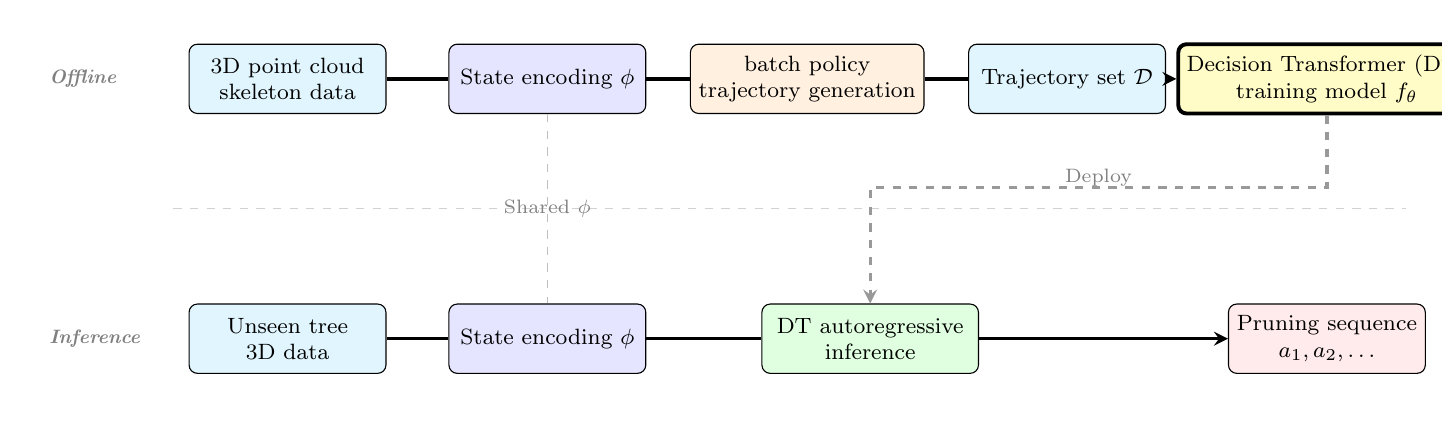
\begin{tikzpicture}[
  bx/.style={rectangle, draw, minimum width=2.5cm, minimum height=0.88cm,
             align=center, font=\footnotesize, rounded corners=3pt, inner sep=3pt},
  bxwide/.style={bx, minimum width=2.75cm},
  arr/.style={->, >=stealth, line width=1.2pt},
  das/.style={->, >=stealth, line width=1.2pt, dashed, gray!80},
]
% Expand bounding box so left labels are not clipped by resizebox
\path[use as bounding box] (0, 0.35) rectangle (17.6, 5.15);

% ---- Offline row (y = 4.5) ----
\node[bx, fill=cyan!12]   (d1) at (3.3,  4.5) {3D point cloud\\skeleton data};
\node[bx, fill=blue!10]   (d2) at (6.6,  4.5) {State encoding $\phi$};
\node[bx, fill=orange!12] (d3) at (9.9,  4.5) {batch policy\\trajectory generation};
\node[bx, fill=cyan!12]   (d4) at (13.2, 4.5) {Trajectory set $\mathcal{D}$};
\node[bx, fill=yellow!22, line width=1.4pt] (d5) at (16.5, 4.5)
  {Decision Transformer (DT)\\training model $f_\theta$};

\draw[arr] (d1)--(d2) (d2)--(d3) (d3)--(d4) (d4)--(d5);

% ---- Inference row (y = 1.2): i4 under d5, i3 between d3--d4 ----
\node[bx, fill=cyan!12]   (i1) at (3.3,  1.2) {Unseen tree\\3D data};
\node[bx, fill=blue!10]   (i2) at (6.6,  1.2) {State encoding $\phi$};
\node[bxwide, fill=green!12] (i3) at (10.7, 1.2)
  {DT autoregressive\\inference};
\node[bx, fill=red!8]     (i4) at (16.5, 1.2) {Pruning sequence\\$a_1,a_2,\ldots$};

\draw[arr] (i1)--(i2) (i2)--(i3) (i3)--(i4);

% ---- Phase labels (anchor=west: text grows rightward, kept clear of d1/i1) ----
\node[font=\scriptsize\bfseries, gray, anchor=west] at (0.15, 4.5) {\textit{Offline}};
\node[font=\scriptsize\bfseries, gray, anchor=west] at (0.15, 1.2) {\textit{Inference}};

% ---- Phase separator ----
\draw[gray!35, thin, dashed] (1.85, 2.85) -- (17.5, 2.85);

% ---- Shared $\phi$ ----
\draw[gray!50, thin, dashed] (d2.south)--(i2.north);
\node[font=\scriptsize, gray] at (6.6, 2.85) {Shared $\phi$};

% ---- Deploy (L-shaped, same as Chinese version) ----
\draw[das] (d5.south) -- (16.5, 3.12) -- (10.7, 3.12) -- (i3.north);
\node[font=\scriptsize, gray] at (13.6, 3.24) {Deploy};

\end{tikzpicture}%
}
\caption{Overall system pipeline}
\label{fig:pipeline}
\end{figure}

\subsection{Data Preprocessing and Safety Constraints}\label{sec:model:preprocess}

\subsubsection{3D Data Preprocessing}

Raw lemon-tree scan data consist of point cloud files and skeleton files.

The dataset is split at the tree-instance level into training and test sets (85\%/15\%),
ensuring that data from the same tree do not appear in both sets,
thereby avoiding data leakage and validating generalization to unseen trees.

\subsubsection{Three-Level Safety Constraints}

Fruit-tree pruning involves irreversible operations on three-dimensional structure;
three-level safety constraints are introduced during trajectory generation.

\textbf{Root-branch protection.}
By traversing the parent-node index of each node in the skeleton data,
the set of branches $\mathcal{B}_{\text{root}}$ with no parent branch is identified,
i.e., the root branches of the tree (typically the trunk and bases of primary scaffolds).
Root branches may not be selected for removal at any time.

\textbf{Minimum structure constraint.}
Let $N_s$ denote the total number of skeleton nodes at the current step.
After removing branch $b$ and all its descendant branches $\operatorname{desc}(b)$,
the remaining node count must satisfy:
\begin{equation}\label{eq:min_structure}
  N_s^{\text{after}} \geq \max\!\left(10,\; \lfloor 0.1 \cdot N_s \rfloor\right)
\end{equation}
This constraint prevents excessive pruning from degrading the skeleton into an irrecoverable residual structure.

\textbf{Protected-branch integrity check.}
Before each candidate removal is executed,
it is verified that all protected branches $\mathcal{B}_{\text{root}}$ still exist in the remaining skeleton.
If any protected branch disappears due to cascaded removal, the operation is rejected.
This check ensures preservation of the basic skeletal framework throughout trajectory generation.

The three constraints are applied in sequence before each action,
forming a constraint chain from root-branch protection to overall structural preservation.


\subsection{Offline Trajectory Construction}\label{sec:model:dataset}

\subsubsection{Random-Policy Trajectory Generation}

At each step, the random policy uniformly samples an action from the currently prunable branches (excluding protected branches).
The target pruning fraction of each trajectory is uniformly sampled from $[0.2, 0.3]$,
thereby covering both light and moderate pruning regimes.
Termination occurs when the cumulative pruning fraction reaches the trajectory target or the hard upper bound $\eta_{\max}=0.30$.

After each step, the composite reward function defined in Section~\ref{sec:formalization:reward}
is used to compute the immediate reward $r_t$.
A termination action $\texttt{STOP}$ is appended at the end of each trajectory.

The random policy is used mainly to broaden the data distribution.
Although such trajectories yield lower overall return on average,
they cover state regions less frequently visited by the heuristic expert policy,
thereby providing necessary contrast samples for subsequent policy learning.

Taking sample Lemon00\_01 as an example, one trajectory generated by the random policy is shown in \cref{tab:random_traj_example}.
The complete trajectory contains $T = 167$ time steps (the first 166 steps are pruning actions, and step 167 is the termination action $\texttt{STOP}$),
with target pruning fraction $0.264$,
cumulative return $\sum_{t=0}^{T-1} r_t = 22.09$,
and cumulative pruning fraction at termination $\eta_{T-1} = 0.263$.

\begin{table}[H]
\centering
\small
\setlength{\tabcolsep}{6pt}
\renewcommand{\arraystretch}{1.15}
\begin{tabular}{rcrrrrr}
\toprule
$t$ & $a_t$ & \old{$r_t$} & \old{$\hat{R}_t$} & $|\mathcal{P}_t|$ & $|\mathcal{S}_t|$ & $\eta_t$ \\
\midrule
0   & 26           & \old{0.089} & \old{22.094} & 56\,742 & 6\,225 & 0.002 \\
1   & 283          & \old{0.027} & \old{22.004} & 56\,608 & 6\,210 & 0.003 \\
2   & 252          & \old{0.125} & \old{21.977} & 56\,556 & 6\,203 & 0.005 \\
\multicolumn{7}{c}{$\cdots$} \\
62  & 427          & \old{0.142} & \old{14.007} & 52\,341 & 5\,691 & 0.100 \\
125 & 465          & \old{0.138} & \old{6.151}  & 47\,323 & 5\,122 & 0.200 \\
\multicolumn{7}{c}{$\cdots$} \\
164 & 168          & \old{0.068} & \old{0.296}  & 43\,316 & 4\,677 & 0.262 \\
165 & 607          & \old{0.228} & \old{0.228}  & 43\,262 & 4\,671 & 0.264 \\
166 & \texttt{STOP}& \old{0.000} & \old{0.000}  & 43\,178 & 4\,658 & 0.264 \\
\bottomrule
\end{tabular}
\caption{Offline trajectory from the random policy on a single sample}
\label{tab:random_traj_example}
\vspace{2pt}

\small Note: $a_t$ is the removed branch ID or termination; \old{$r_t$ and $\hat{R}_t$ are immediate reward and return-to-go;}
$|\mathcal{P}_t|$ and $|\mathcal{S}_t|$ are pre-pruning point-cloud and current skeleton sizes; $\eta_t$ is the cumulative pruning fraction.\\
\rev{Note: the two struck-through columns are retained for transparency only and are no longer reported. Their values were produced by an earlier reward-function version whose scale differs from the composite reward defined in Section~\ref{sec:formalization:reward}; they will be recomputed after the full-scale experiments.}
\end{table}


\subsubsection{Heuristic Expert-Policy Trajectory Generation}

The heuristic expert policy scores all prunable branches of the current tree at each step according to branch discrimination rules, protection rules, and reward design,
and selects the action with the highest composite score.
The scoring rules are consistent with the branch quality reward in the composite reward function:

\begin{itemize}[nosep]
  \item Crossing branches: tiered proportional rewards by severity $\sigma$
  \item Inner shaded branches and upright water sprouts: higher positive rewards
  \item Pendulous branches and weak branches: moderate and lower positive rewards, respectively
  \item Medium-short branch protection and sturdy branch protection: negative rewards, with stronger penalty for the latter
\end{itemize}

In addition, the expert policy introduces a penalty term proportional to removal volume, $-\lambda_{\text{exp}} V_b$,
to avoid removing an oversized subtree in a single step.
When the composite score of all candidate branches is below zero,
the policy determines that no further pruning is needed and terminates automatically.
For the same tree state, the action choice remains consistent,
and each step can be traced back to specific branch discrimination grounds.
The automatic termination mechanism suppresses unnecessary continued pruning.
Expert trajectories typically yield higher cumulative return
and provide high-quality samples for training.

Taking sample Lemon00\_01 as an example, one trajectory generated by the expert policy is shown in \cref{tab:expert_traj_example}.
The complete trajectory contains $T = 190$ time steps (the first 189 steps are pruning actions, and step 190 is the termination action $\texttt{STOP}$),
with cumulative return $\sum_{t=0}^{T-1} r_t = 39.49$,
and cumulative pruning fraction at termination $\eta_{T-1} = 0.300$.

\begin{table}[H]
\centering
\small
\setlength{\tabcolsep}{6pt}
\renewcommand{\arraystretch}{1.15}
\begin{tabular}{rcrrrrr}
\toprule
$t$ & $a_t$ & \old{$r_t$} & \old{$\hat{R}_t$} & $|\mathcal{P}_t|$ & $|\mathcal{S}_t|$ & $\eta_t$ \\
\midrule
0   & 626          & \old{0.246} & \old{39.487} & 56\,742 & 6\,225 & 0.002 \\
1   & 620          & \old{0.243} & \old{39.241} & 56\,690 & 6\,219 & 0.003 \\
2   & 591          & \old{0.281} & \old{38.998} & 56\,641 & 6\,213 & 0.005 \\
\multicolumn{7}{c}{$\cdots$} \\
36  & 615          & \old{0.360} & \old{31.065} & 54\,647 & 5\,966 & 0.059 \\
62  & 443          & \old{0.209} & \old{25.002} & 52\,480 & 5\,739 & 0.100 \\
125 & 595          & \old{0.333} & \old{11.949} & 47\,623 & 5\,189 & 0.200 \\
\multicolumn{7}{c}{$\cdots$} \\
187 & 554          & \old{0.148} & \old{0.254}  & 43\,565 & 4\,672 & 0.298 \\
188 & 257          & \old{0.106} & \old{0.106}  & 43\,529 & 4\,666 & 0.300 \\
189 & \texttt{STOP}& \old{0.000} & \old{0.000}  & 43\,475 & 4\,659 & 0.300 \\
\bottomrule
\end{tabular}
\caption{Offline trajectory from the expert policy on a single sample}
\label{tab:expert_traj_example}
\vspace{2pt}

\small Note: $a_t$ is the removed branch ID or termination; \old{$r_t$ and $\hat{R}_t$ are immediate reward and return-to-go;}
$|\mathcal{P}_t|$ and $|\mathcal{S}_t|$ are pre-pruning point-cloud and current skeleton sizes; $\eta_t$ is the cumulative pruning fraction.\\
\rev{Note: the two struck-through columns are retained for transparency only and are no longer reported. Their values were produced by an earlier reward-function version whose scale differs from the composite reward defined in Section~\ref{sec:formalization:reward}; they will be recomputed after the full-scale experiments.}
\end{table}

The training dataset is formed by directly merging random-policy and expert-policy trajectories,
without weighting or oversampling.


\subsection{Trajectory Representation and Sequence Modeling}\label{sec:model:formulation}

\subsubsection{State Encoding}

The tree state at each step is jointly represented by the current point cloud and skeleton.
The point cloud provides a dense three-dimensional spatial distribution,
while the skeleton encodes sparse but topologically explicit structural relations.
To fuse the two modalities, a dual-path encoder $\phi: (\mathcal{P}, \mathcal{S}) \to \mathbb{R}^{d_s}$ is adopted,
mapping variable-length 3D structural data to a fixed-dimensional state vector $s_t \in \mathbb{R}^{d_s}$ ($d_s = 64$).
\Cref{fig:encoder,tab:encoder_config} present the architecture and module configuration of the state encoder.

\begin{figure}[htbp]
\centering
\resizebox{0.98\linewidth}{!}{%
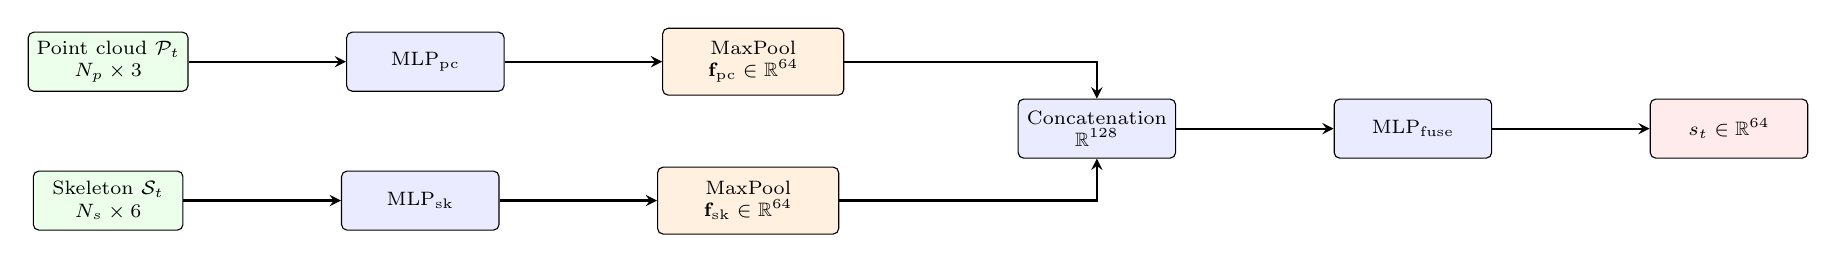
\begin{tikzpicture}[
  node distance=1.0cm and 2.0cm,
  block/.style={rectangle, draw, fill=blue!8, minimum width=2.0cm, minimum height=0.75cm,
                font=\scriptsize, align=center, rounded corners=2pt, inner sep=3pt},
  data/.style={rectangle, draw, fill=green!8, minimum width=1.9cm, minimum height=0.75cm,
               font=\scriptsize, align=center, rounded corners=2pt, inner sep=3pt},
  pool/.style={rectangle, draw, fill=orange!12, minimum width=2.3cm, minimum height=0.85cm,
               font=\scriptsize, align=center, rounded corners=2pt, inner sep=3pt},
  output/.style={rectangle, draw, fill=red!8, minimum width=2.0cm, minimum height=0.75cm,
                 font=\scriptsize, align=center, rounded corners=2pt, inner sep=3pt},
  arr/.style={->, >=stealth, thick},
]
  \node[data] (pc) {Point cloud $\mathcal{P}_t$\\$N_p \times 3$};
  \node[data, below=of pc] (sk) {Skeleton $\mathcal{S}_t$\\$N_s \times 6$};

  \node[block, right=of pc] (mlp_pc) {$\text{MLP}_{\text{pc}}$};
  \node[block, right=of sk] (mlp_sk) {$\text{MLP}_{\text{sk}}$};

  \node[pool, right=of mlp_pc] (pool_pc) {MaxPool\\$\mathbf{f}_{\text{pc}} \in \mathbb{R}^{64}$};
  \node[pool, right=of mlp_sk] (pool_sk) {MaxPool\\$\mathbf{f}_{\text{sk}} \in \mathbb{R}^{64}$};

  \node[block, right=2.2cm of pool_pc, yshift=-0.85cm] (concat) {Concatenation\\$\mathbb{R}^{128}$};
  \node[block, right=of concat] (fuse) {$\text{MLP}_{\text{fuse}}$};
  \node[output, right=of fuse] (out) {$s_t \in \mathbb{R}^{64}$};

  \draw[arr] (pc) -- (mlp_pc);
  \draw[arr] (sk) -- (mlp_sk);
  \draw[arr] (mlp_pc) -- (pool_pc);
  \draw[arr] (mlp_sk) -- (pool_sk);
  \draw[arr] (pool_pc) -| (concat);
  \draw[arr] (pool_sk) -| (concat);
  \draw[arr] (concat) -- (fuse);
  \draw[arr] (fuse) -- (out);
\end{tikzpicture}%
}
\caption{Dual-path fused state encoder architecture}
\label{fig:encoder}
\end{figure}

\begin{table}[H]
\centering
\small
\begin{tabular}{llll}
\toprule
\textbf{Module} & \textbf{Input dim.} & \textbf{Hidden layer} & \textbf{Output dim.} \\
\midrule
$\text{MLP}_{\text{pc}}$ (point cloud path) & 3 & 64 (ReLU) & 64 \\
$\text{MLP}_{\text{sk}}$ (skeleton path) & 6 & 64 (ReLU) & 64 \\
Global max pooling & $N \times 64$ & --- & 64 \\
$\text{MLP}_{\text{fuse}}$ (fusion layer) & 128 & 128 (ReLU) & 64 \\
\bottomrule
\end{tabular}
\caption{Module configuration of the state encoder}
\label{tab:encoder_config}
\end{table}

The encoder adopts a dual-path parallel structure,
extracting per-point features from the point cloud and skeleton through separate MLPs,
then aggregating them via global max pooling into fixed-dimensional global representations.
The two global features are concatenated and mapped by the fusion layer to the final state vector:
\begin{equation}\label{eq:state_encode}
  s_t = \phi(\mathcal{P}_t, \mathcal{S}_t) =
    \text{MLP}_{\text{fuse}}\!\left(
      \left[\text{MaxPool}\!\left(\text{MLP}_{\text{pc}}(\mathcal{P}_t)\right) \;\big\|\;
       \text{MaxPool}\!\left(\text{MLP}_{\text{sk}}(\mathcal{S}_t)\right)\right]
    \right)
\end{equation}
where $[\cdot \| \cdot]$ denotes vector concatenation.
Global max pooling makes the encoder invariant to input point ordering
and compresses variable-length inputs into fixed-length representations for subsequent Transformer input.

\subsubsection{Serialized Trajectory Representation}

A pruning trajectory consists of raw observations, actions, and immediate rewards at each step.
Under the conditional sequence generation framework of Decision Transformer,
the trajectory is further written in a form that includes return-to-go (RTG).

RTG is defined as the cumulative return from the current time step to the end of the trajectory:
\begin{equation}\label{eq:rtg}
  \hat{R}_t = \sum_{k=t}^{T-1} r_k
\end{equation}
$\hat{R}_t$ characterizes the cumulative reward still obtainable after the current time step,
corresponding to the target-return condition at that step for the model.


The sequence modeling objective is:
given target return $\hat{R}_t$, historical state sequence $s_{\leq t}$, and historical action sequence $a_{<t}$,
predict the optimal action at the current time step:
\begin{equation}\label{eq:seq_model}
  \hat{a}_t = \arg\max\; f_\theta\!\left(\hat{R}_{\leq t},\; s_{\leq t},\; a_{<t}\right)
\end{equation}
where $f_\theta$ is the parameterized sequence model.


\subsection{Decision Transformer Model}\label{sec:model:dt}

Decision Transformer~\citep{chen2021decision} reformulates offline reinforcement learning
as a conditional sequence generation problem,
using an autoregressive Transformer to generate actions from desired return and historical trajectories.
Compared with traditional offline RL methods that must explicitly handle distributional shift and value-function estimation (e.g.,
BCQ~\citep{fujimoto2019bcq}, CQL~\citep{kumar2020conservative}),
this framework addresses decision making through sequence modeling,
and is suited to discrete decision settings such as ours, where the action space changes with tree state.

In this work, the backbone of Decision Transformer follows the standard causal sequence modeling framework,
but its input representation and decision objects are specialized for the fruit-tree pruning task.
Model inputs consist of interleaved tokens of return-to-go, tree state, and historical actions,
where state tokens are given by $s_t$ from the dual-path point-cloud and skeleton encoder,
and action tokens correspond to discrete pruning actions on the current tree and the termination action $\texttt{STOP}$.
This representation enables joint modeling of target constraints, structural state, and historical decisions within one sequence.

Decision Transformer is adopted because fruit-tree pruning exhibits pronounced long-horizon temporal dependence:
earlier actions continuously alter the subsequent set of prunable branches and the overall tree structure.
Meanwhile, return conditioning provides adjustable optimization preferences at inference,
helping the model balance structural hierarchy, interior canopy openness, and fruit-bearing potential protection.
Therefore, it serves as the offline sequential decision model in this paper,
and its ability to model pruning trajectories is examined under the above task setting.
\Cref{fig:dt_arch} illustrates the input--output form of the Decision Transformer model.

\begin{figure}[htbp]
\centering
\resizebox{\linewidth}{!}{%
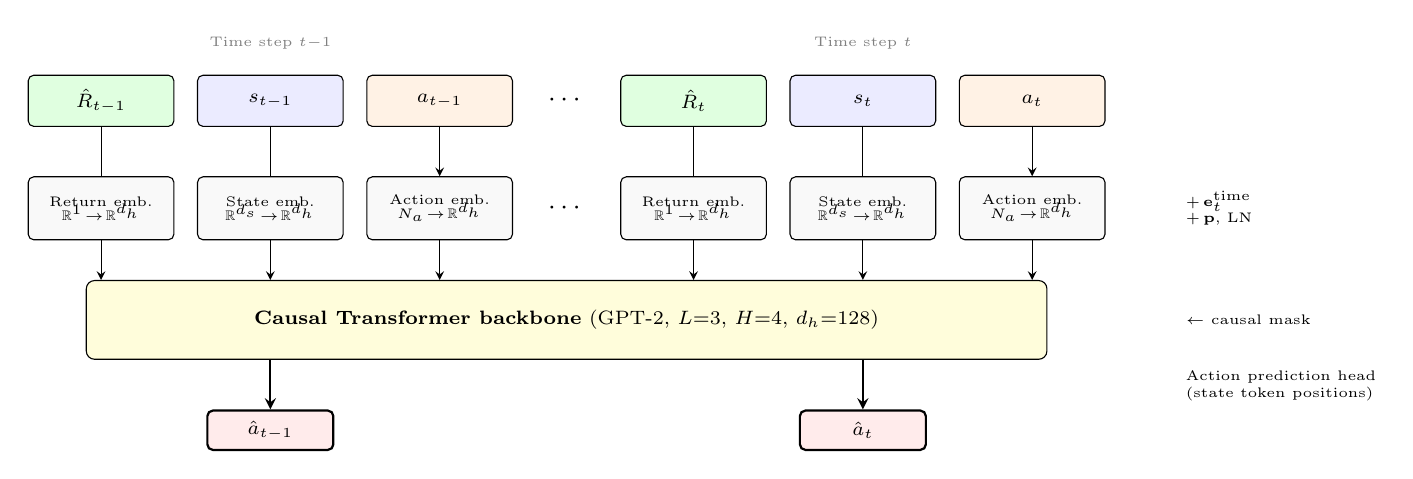
\begin{tikzpicture}[
  x=2.15cm, y=1.05cm,
  tok/.style={rectangle, draw, minimum width=1.85cm, minimum height=0.65cm,
              align=center, font=\scriptsize, rounded corners=2pt, inner sep=2pt},
  rtg/.style={tok, fill=green!12},
  stt/.style={tok, fill=blue!8},
  act/.style={tok, fill=orange!10},
  emb/.style={rectangle, draw, minimum width=1.85cm, minimum height=0.8cm,
              align=center, font=\tiny, fill=gray!5, rounded corners=2pt, inner sep=2pt},
  trm/.style={rectangle, draw, fill=yellow!14, minimum height=1.0cm,
              align=center, font=\scriptsize, rounded corners=3pt, inner sep=4pt},
  hed/.style={rectangle, draw, fill=red!8, minimum width=1.6cm, minimum height=0.5cm,
              align=center, font=\scriptsize, rounded corners=2pt},
  arr/.style={->, >=stealth, thin},
  harr/.style={->, >=stealth, thick},
]

% --- Time-step labels ---
\node[font=\tiny, gray] at (1, 4.2) {Time step $t{-}1$};
\node[font=\tiny, gray] at (4.5, 4.2) {Time step $t$};

% --- Token row ---
\node[rtg] (r1) at (0, 3.5)  {$\hat{R}_{t-1}$};
\node[stt] (s1) at (1, 3.5)  {$s_{t-1}$};
\node[act] (a1) at (2, 3.5)  {$a_{t-1}$};
\node      at (2.75, 3.5)    {$\cdots$};
\node[rtg] (r2) at (3.5, 3.5)  {$\hat{R}_t$};
\node[stt] (s2) at (4.5, 3.5)  {$s_t$};
\node[act] (a2) at (5.5, 3.5) {$a_t$};

% --- Embedding row ---
\node[emb] (re1) at (0, 2.2)  {Return emb.\\[-1pt]$\mathbb{R}^1\!\to\!\mathbb{R}^{d_h}$};
\node[emb] (se1) at (1, 2.2)  {State emb.\\[-1pt]$\mathbb{R}^{d_s}\!\to\!\mathbb{R}^{d_h}$};
\node[emb] (ae1) at (2, 2.2)  {Action emb.\\[-1pt]$N_a\!\to\!\mathbb{R}^{d_h}$};
\node      at (2.75, 2.2)      {$\cdots$};
\node[emb] (re2) at (3.5, 2.2)  {Return emb.\\[-1pt]$\mathbb{R}^1\!\to\!\mathbb{R}^{d_h}$};
\node[emb] (se2) at (4.5, 2.2)  {State emb.\\[-1pt]$\mathbb{R}^{d_s}\!\to\!\mathbb{R}^{d_h}$};
\node[emb] (ae2) at (5.5, 2.2) {Action emb.\\[-1pt]$N_a\!\to\!\mathbb{R}^{d_h}$};

\draw[arr] (r1)--(re1) (s1)--(se1) (a1)--(ae1);
\draw[arr] (r2)--(re2) (s2)--(se2) (a2)--(ae2);

% Embedding annotation (right)
\node[font=\tiny, align=left, anchor=west] at (6.35, 2.2)
  {$+\,\mathbf{e}_t^{\mathrm{time}}$\\$+\,\mathbf{p}$, LN};

% --- Transformer backbone ---
\node[trm, minimum width=12.2cm] (trm) at (2.75, 0.85)
  {\textbf{Causal Transformer backbone} (GPT-2, $L{=}3$, $H{=}4$, $d_h{=}128$)};

\draw[arr] (re1.south)--(re1.south |- trm.north);
\draw[arr] (se1.south)--(se1.south |- trm.north);
\draw[arr] (ae1.south)--(ae1.south |- trm.north);
\draw[arr] (re2.south)--(re2.south |- trm.north);
\draw[arr] (se2.south)--(se2.south |- trm.north);
\draw[arr] (ae2.south)--(ae2.south |- trm.north);

% --- Action prediction ---
\draw[harr] (se1.south |- trm.south) -- ++(0,-0.6)
  node[hed, below] {$\hat{a}_{t-1}$};
\draw[harr] (se2.south |- trm.south) -- ++(0,-0.6)
  node[hed, below] {$\hat{a}_t$};

% Annotations
\node[font=\tiny, anchor=west] at (6.35, 0.85) {$\leftarrow$ causal mask};
\node[font=\tiny, align=left, anchor=west] at (6.35, 0.05)
  {Action prediction head\\(state token positions)};

\end{tikzpicture}%
}
\caption{Illustration of Decision Transformer input--output form for fruit-tree pruning (two adjacent time steps)}
\label{fig:dt_arch}
\end{figure}

\subsubsection{Training and Inference}

During training, standard multi-class cross-entropy loss is used:
\begin{equation}\label{eq:dt_loss}
  \mathcal{J}_{\mathrm{CE}} = -\frac{1}{|\mathcal{M}|} \sum_{t \in \mathcal{M}}
    \log \frac{\exp(\mathbf{z}_t[a_t^*])}{\sum_{j=1}^{N_a} \exp(\mathbf{z}_t[j])}
\end{equation}
where $\mathcal{J}_{\mathrm{CE}}$ is the cross-entropy training objective, $\mathcal{M}$ is the set of non-padded positions, $\mathbf{z}_t$ is the action logits at time step $t$,
and $a_t^*$ is the ground-truth action in the trajectory.

The optimizer is AdamW,
with a linear warmup scheduler.
The gradient clipping threshold is 1.0, batch size is 32, and training runs for 1000 epochs.
\Cref{tab:dt_config} reports the hyperparameter configuration of the Decision Transformer model.

\begin{table}[H]
\centering
\begin{tabular}{llc}
\toprule
\textbf{Category} & \textbf{Hyperparameter} & \textbf{Value} \\
\midrule
\multirow{4}{*}{Model architecture}
  & State dimension $d_s$ & 64 \\
  & Hidden dimension $d_h$ & 128 \\
  & Transformer layers & 3 \\
  & Attention heads & 4 \\
\addlinespace
\multirow{3}{*}{Regularization}
  & Attention dropout & 0.1 \\
  & Residual dropout & 0.1 \\
  & Embedding dropout & 0.1 \\
\addlinespace
\multirow{5}{*}{Training}
  & Learning rate & $10^{-4}$ \\
  & Optimizer & AdamW \\
  & Weight decay & $10^{-4}$ \\
  & Warmup ratio & 10\% \\
  & Gradient clipping & 1.0 \\
\addlinespace
\multirow{3}{*}{Data}
  & Batch size & 32 \\
  & Max.\ sequence length & Dynamic (95th percentile) \\
  & Point cloud / skeleton cap & 2048 / 256 \\
\bottomrule
\end{tabular}
\caption{Hyperparameter configuration of the Decision Transformer model}
\label{tab:dt_config}
\end{table}

At inference, for unseen trees, the initial target return $\hat{R}_1$ is set to a high percentile of cumulative returns on expert trajectories in the training set.
The model then autoregressively outputs pruning actions step by step; after each step the tree state is updated,
and $\hat{R}_{t+1} = \hat{R}_t - r_t$ is propagated from the actual reward,
until a termination action is output or the maximum number of steps is reached.



% ============================================================
% Chapter 5: Experiments and analysis
% ============================================================
\section{Experiments and Analysis}\label{sec:experiment}
The lemon-tree 3D data used in our experiments are from the TreeNet3D large-scale synthetic tree benchmark dataset~\citep{tang2024treenet3d}.
Each tree provides a mesh model,
branch-level annotated 3D point clouds and noisy point-cloud variants,
together with a complete hierarchical skeleton and tree volume information.
The experiments use 1400 lemon-tree samples as the study objects.
The dataset is split at the tree-instance level into training and test sets (85\%/15\%).
Under this split, the offline trajectory construction stage generates one expert trajectory
and four random trajectories per lemon tree,
five per tree in total, yielding approximately 7000 offline trajectories in the full dataset.
Expert trajectories are used as supervision during model training;
random trajectories expand the state distribution to support dataset statistics and return-conditioning estimation.
For evaluation, four lemon-tree samples with clearly different canopy density, branch complexity, and local crowding are randomly drawn from the test set
as representative individuals for comparative analysis,
helping observe stability of different policies on heterogeneous trees.


\subsection{Benchmark Evaluation}


To compare the sequential decision model with a single-step heuristic policy, this section introduces a greedy baseline based on branch geometric attributes.
For each candidate branch $b$, let $\rho_b$ denote the horizontal distance from branch centroid $\cb$ to the trunk base,
$\alpha_b$ the angle between the branch main axis and the vertical direction $\mathbf{e}_z$,
and $L_b$ the branch length.
Three heuristic scores are defined from these geometric quantities:
\begin{equation}\label{eq:greedy_score}
\begin{aligned}
  s_1(b) &= 1 - \min\!\left(\rho_b / R_t,\; 1\right), \\
  s_2(b) &= \max\!\left(1 - \alpha_b / \alpha_0,\; 0\right), \\
  s_3(b) &= \frac{L_b}{L^{*}} \left(1 - \frac{\rho_b}{\rho^{*}}\right).
\end{aligned}
\end{equation}
where $R_t$ is a constant estimate of the horizontal scale of the tree, $\alpha_0 = 35^\circ$ is the vertical water-sprout angle threshold,
$L^{*} = \max_{b' \in \mathcal{B}_t} L_{b'}$ and $\rho^{*} = \max_{b' \in \mathcal{B}_t} \rho_{b'}$
are normalization factors over the current candidate set $\mathcal{B}_t$.
The three scores measure inward growth tendency ($s_1$), verticality ($s_2$), and long-branch crowding tendency ($s_3$), respectively;
larger values indicate more pronounced geometric features and hence greater tendency for removal.
The composite score is a weighted sum of the three terms:
\begin{equation}\label{eq:greedy_total}
  \mathrm{score}(b) = w_1\,s_1(b) + w_2\,s_2(b) + w_3\,s_3(b),
\end{equation}
At time $t$, the greedy baseline removes the branch with the highest score in the legal candidate set $\mathcal{B}_t$:
\begin{equation}\label{eq:greedy_action}
  b_t^{\,\text{greedy}} = \arg\max_{b \in \mathcal{B}_t}\; \mathrm{score}(b).
\end{equation}
The process terminates when $\max_b \mathrm{score}(b) < \tau_g$ (with $\tau_g = 0.45$)
or the cumulative pruning fraction reaches $\eta_{\max}$.
The greedy baseline and the learned policy use the same evaluation metrics;
the difference is that the former decides via single-step geometric heuristics,
does not use historical trajectory information,
and does not consider how prior actions affect subsequent candidate priorities;
performance differences between the two reflect the contribution of sequence modeling to decision quality.

\begin{figure}[H]
\centering
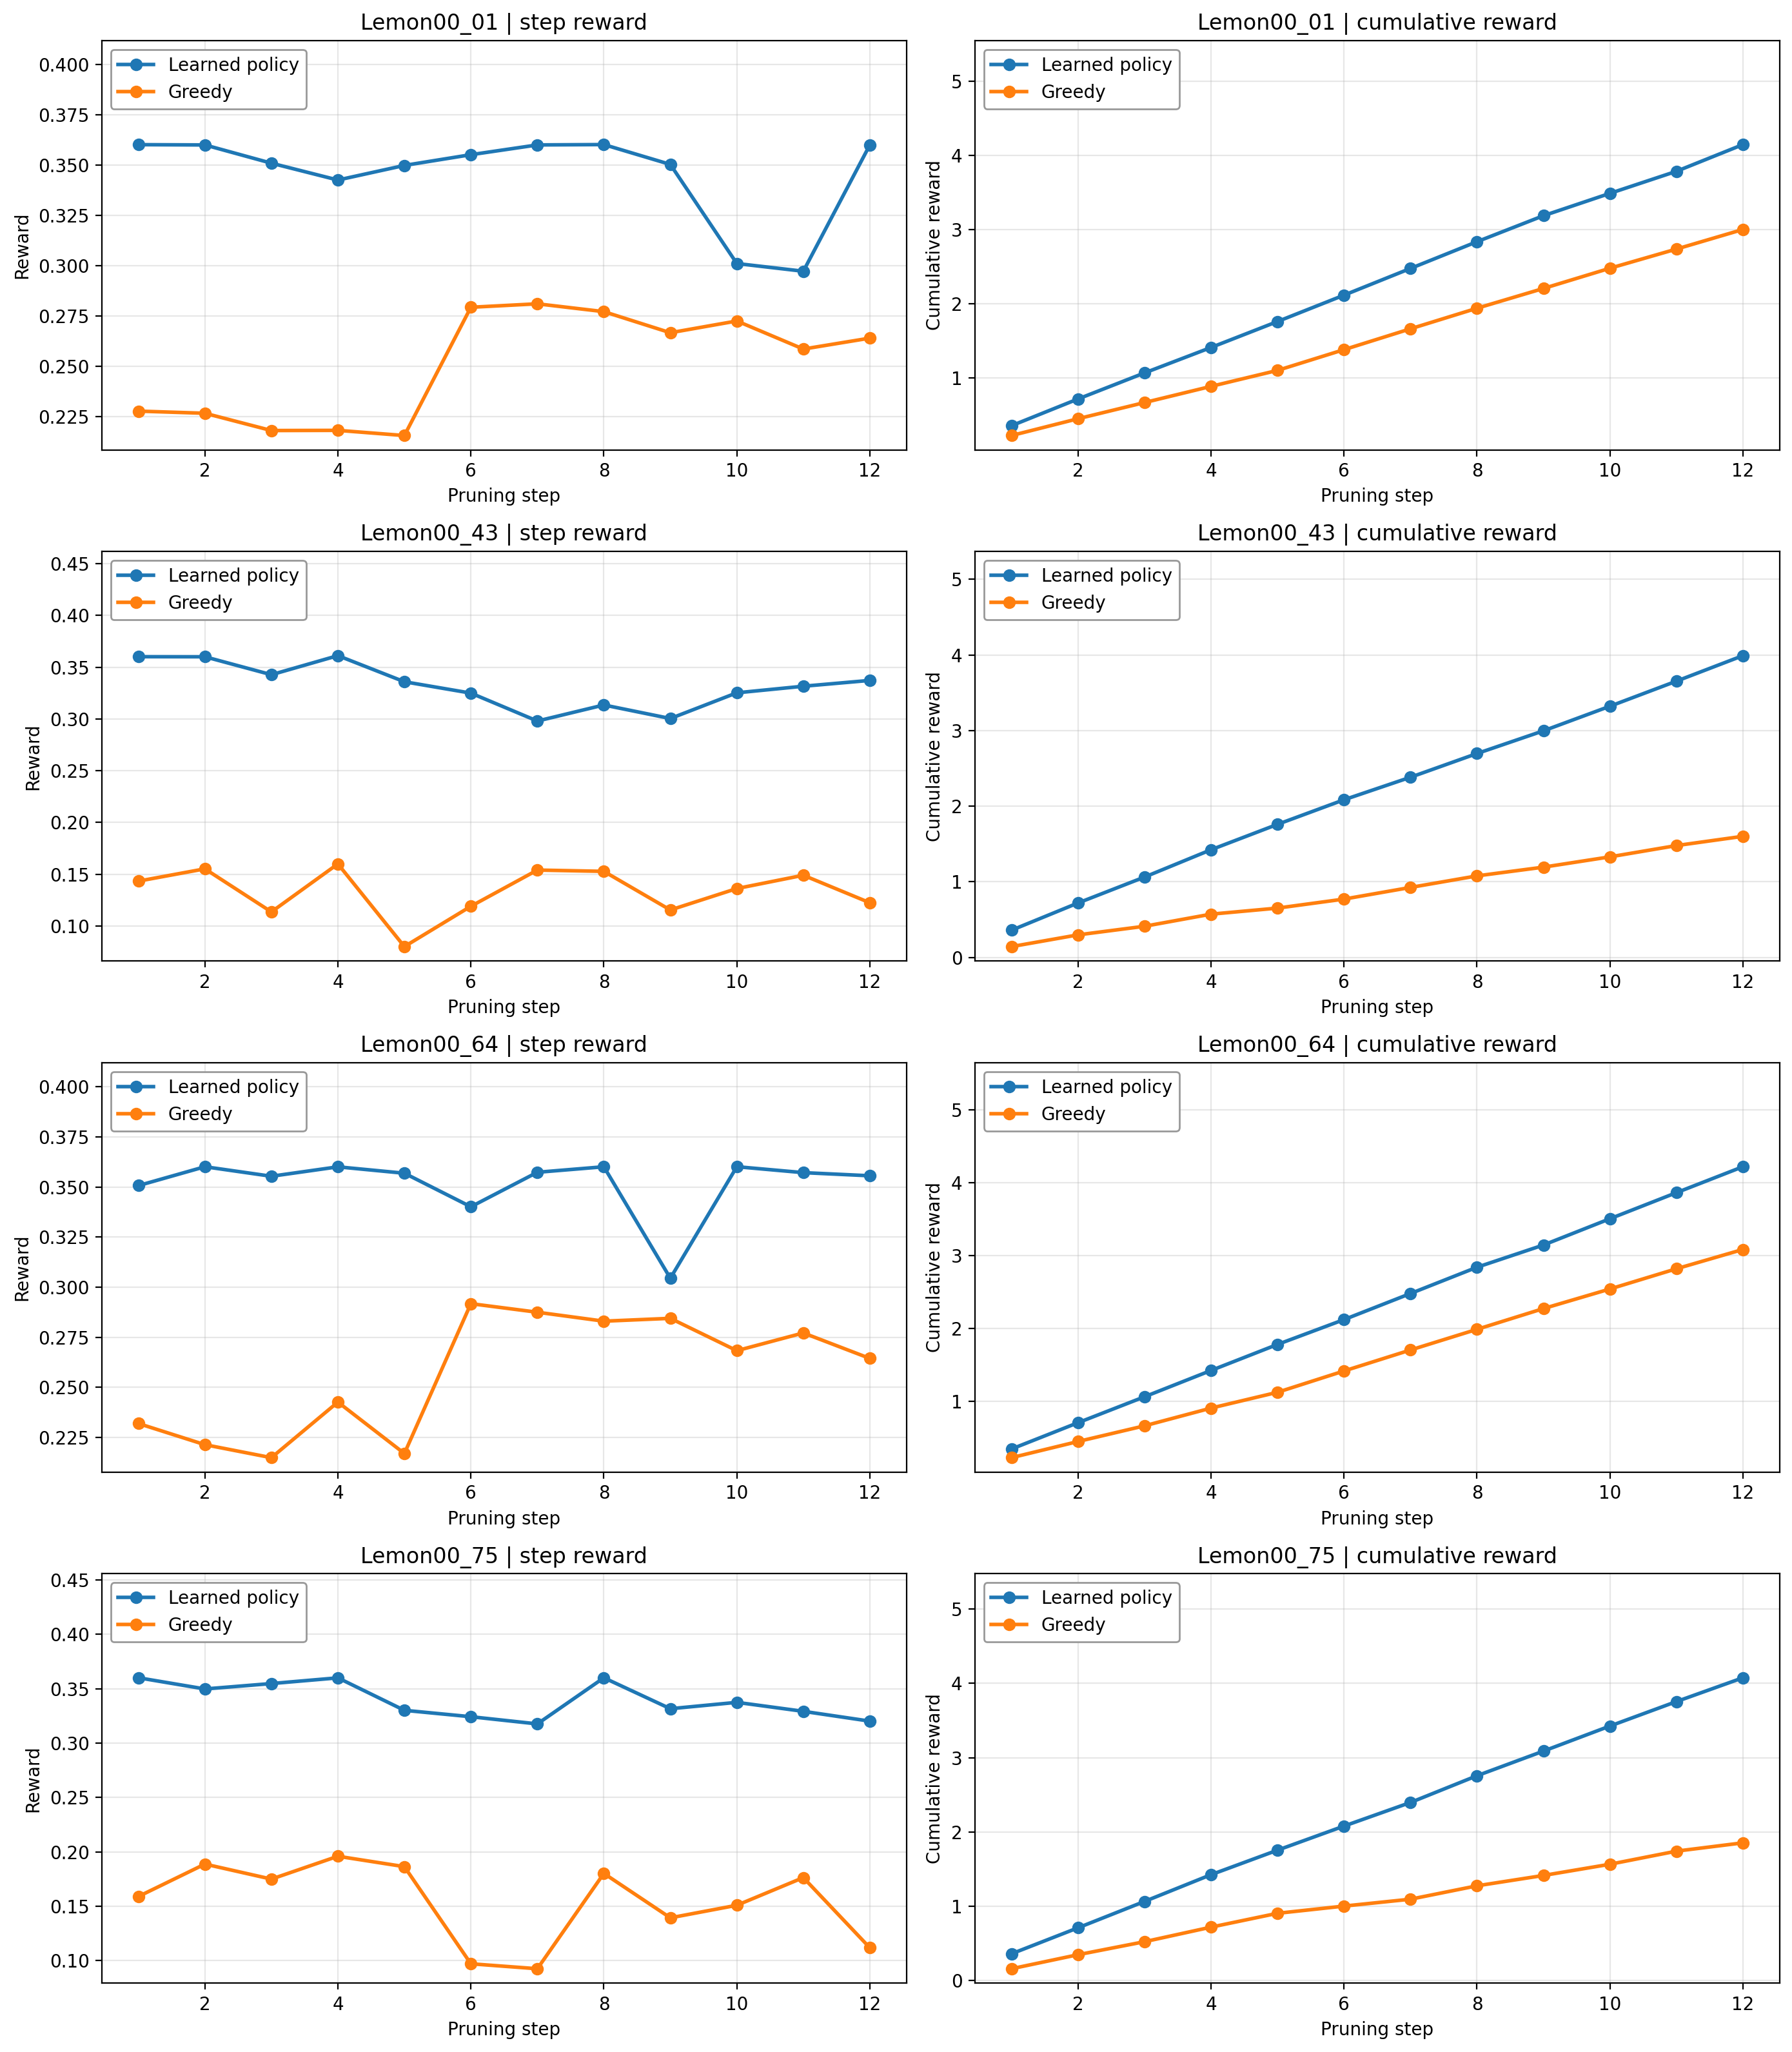
\includegraphics[width=0.85\textwidth]{figures/per_tree_reward.png}
\caption{Per-step and cumulative reward curves on four test samples}
\label{fig:per_tree_reward}
\end{figure}

\begin{figure}[H]
\centering
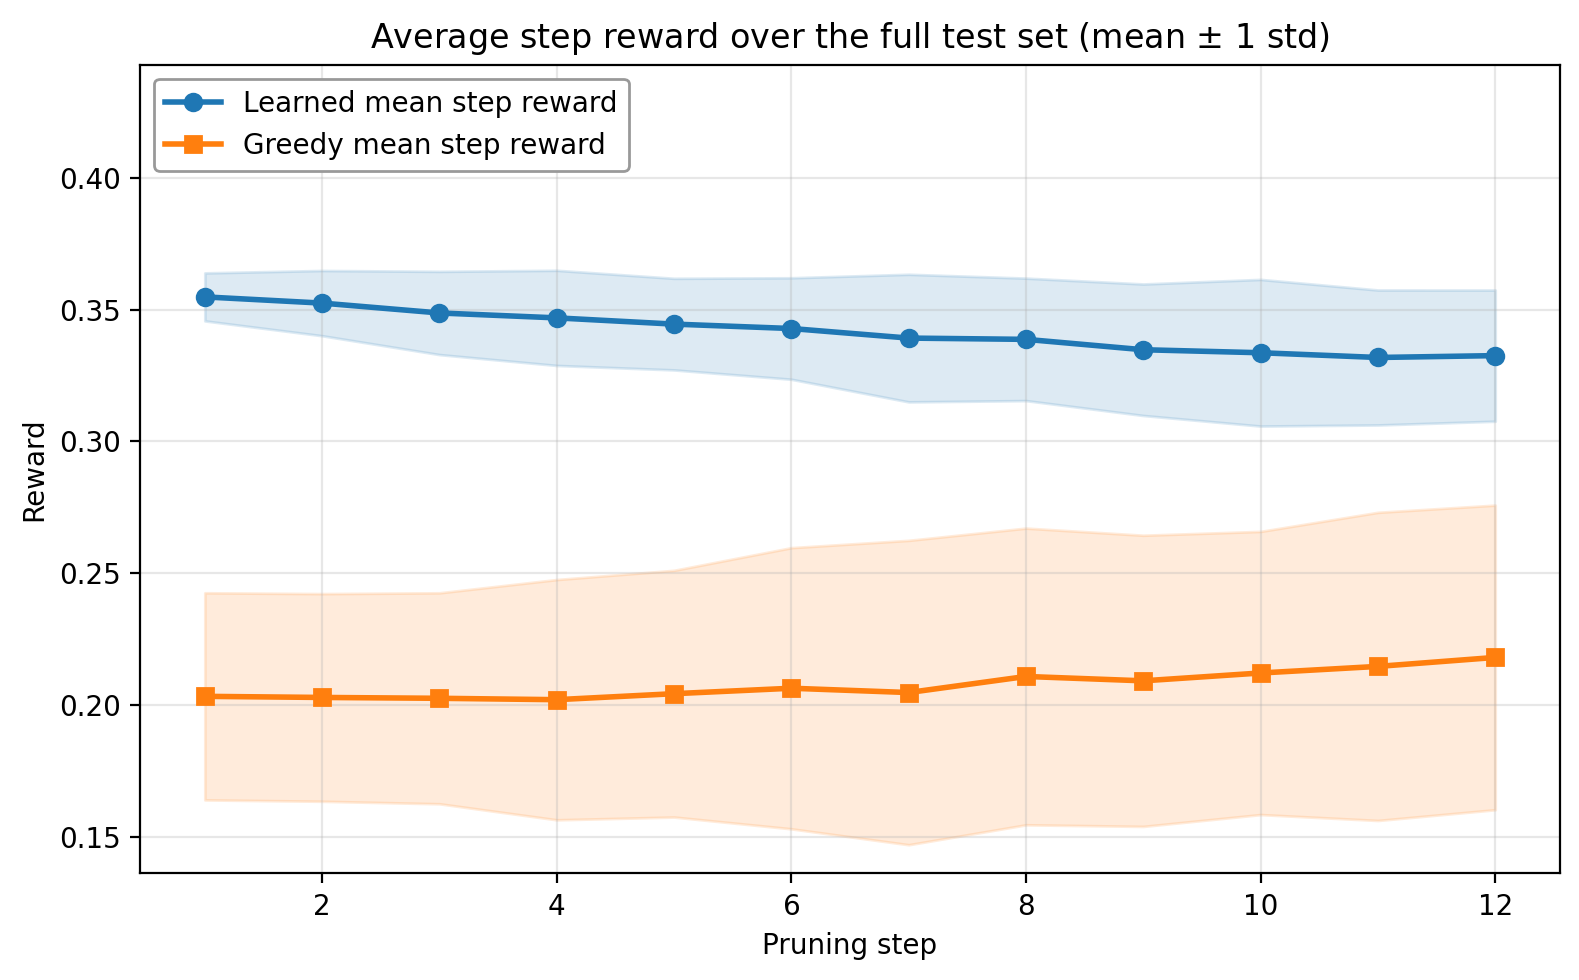
\includegraphics[width=0.75\textwidth]{figures/avg_reward_trend.png}
\caption{Average per-step reward trend}
\label{fig:avg_reward_trend}
\end{figure}

Among the four tree samples in Figure~\ref{fig:per_tree_reward},
with respect to per-step reward, the learned policy shows relatively concentrated reward levels across different trees,
indicating that its action choices do not rely markedly on local geometric idiosyncrasies of any single tree.
The greedy baseline exhibits greater reward fluctuation,
relying only on geometric scores such as current branch centroid distance, vertical angle, and length,
and thus struggling to consistently characterize how removal actions affect subsequent tree state.
As pruning steps increase, the learned policy's cumulative return remains above the greedy baseline,
and the advantage is not confined to the early sequence but continues to accumulate in later actions.

Figure~\ref{fig:avg_reward_trend} aggregates rewards at the same step across approximately 211 trees in the full test set
into mean curves and standard-deviation bands.
The mean curve reflects average immediate return over the overall benchmark,
while the bands reflect dispersion across test trees.
From the mean, the learned policy stays above the greedy baseline throughout the first 12 pruning steps.
The greedy baseline shows limited overall improvement.
Although single-step geometric scoring can select branches with non-negligible reward in some states,
its average return remains below that of the sequence policy learned from offline trajectories.

The greedy baseline's standard-deviation bands are noticeably wider than those of the learned policy at each step,
especially in the middle and late stages,
indicating greater sensitivity to specific canopy morphology and local branch distribution of test trees.
When the same geometric weights are applied to roughly 210 test trees,
similar reward trajectories are difficult to obtain stably.
By contrast, the learned policy's bands are relatively narrower,
indicating better stability of action choices across the full test set.


\begin{figure}[H]
\centering
\begin{subfigure}[t]{0.48\textwidth}
  \centering
  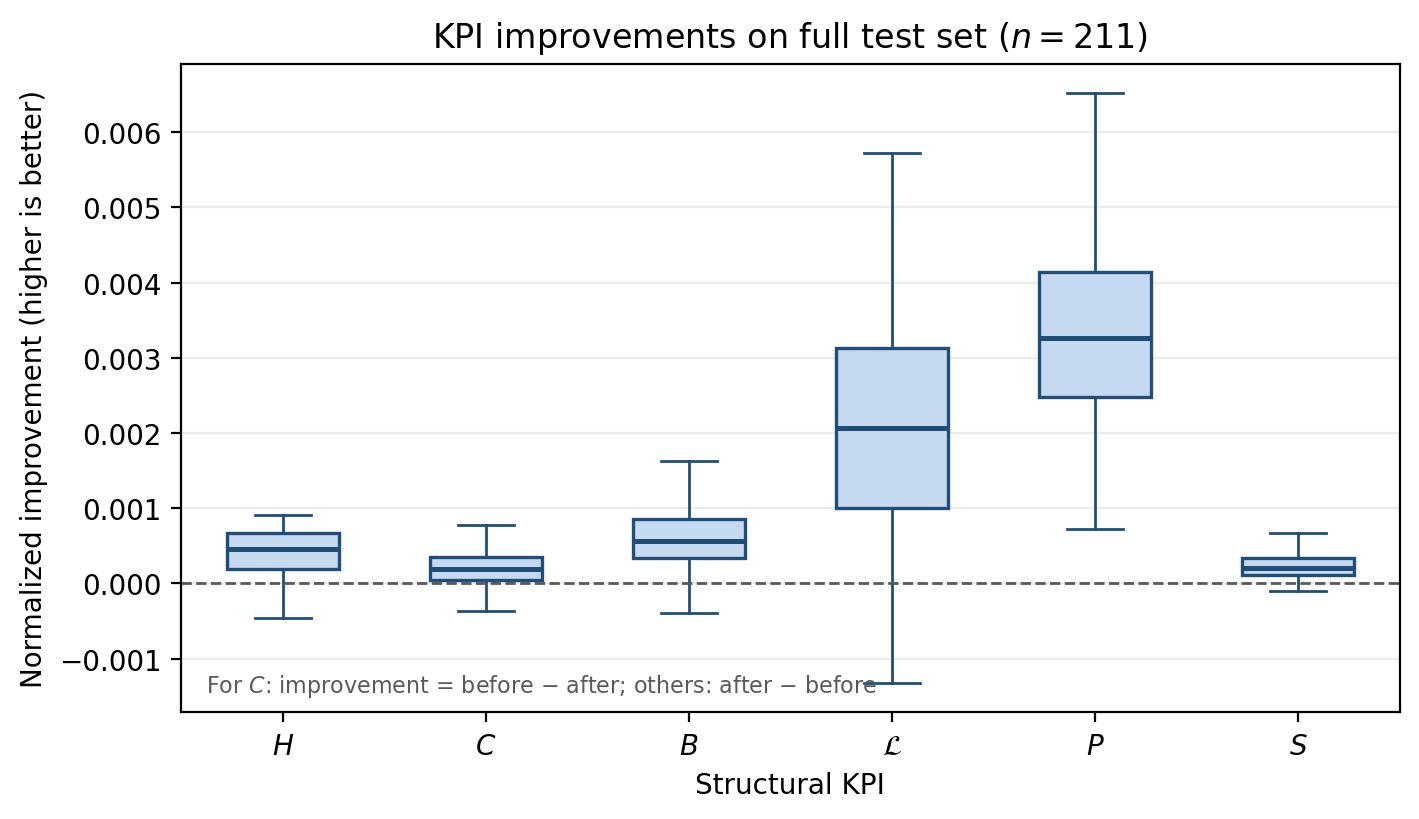
\includegraphics[height=4.6cm,keepaspectratio]{figures/kpi_delta_boxplot.png}
  \caption{Distribution of direction-normalized improvements (outlier points omitted for clarity).}
  \label{fig:kpi_delta_boxplot}
\end{subfigure}
\hfill
\begin{subfigure}[t]{0.48\textwidth}
  \centering
  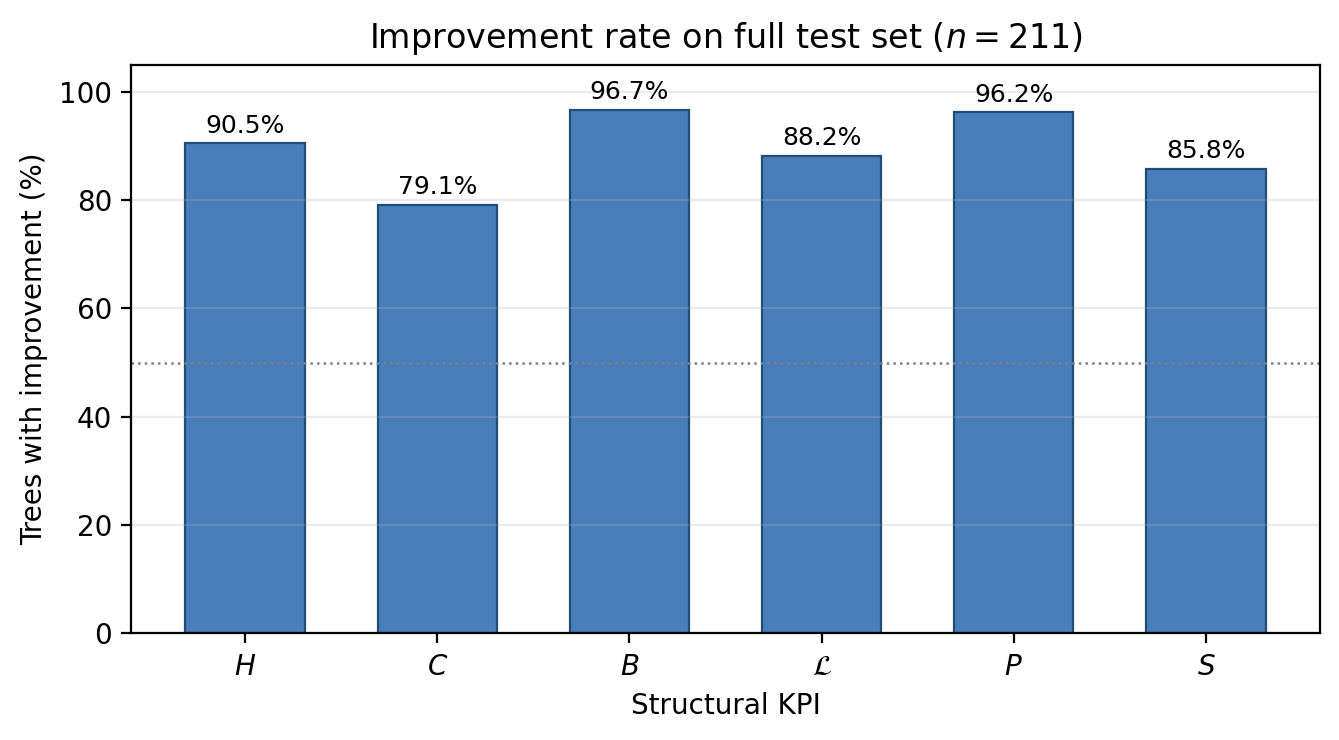
\includegraphics[height=4.6cm,keepaspectratio]{figures/kpi_improvement_rate.png}
  \caption{Proportion of trees with improvement per indicator.}
  \label{fig:kpi_improvement_rate}
\end{subfigure}
\caption{Structural indicator evaluation on the full test set ($n{=}211$)}
\label{fig:kpi_full_test}
\end{figure}

\begin{table}[H]
\centering
\small
\begin{tabular}{lccc}
\toprule
\textbf{Indicator} & \textbf{Before} & \textbf{After} & \textbf{Change} \\
\midrule
Structural hierarchy $H$ & 0.5000 & 0.5000 & 0.0000 \\
Crowding $C$ & 0.5037 & 0.5062 & 0.0025 \\
Balance $B$ & 0.8912 & 0.8927 & 0.0016 \\
Light accessibility $\mathcal{L}$ & 0.3309 & 0.3663 & 0.0354 \\
Fruit-bearing potential $P$ & 0.4286 & 0.4465 & 0.0179 \\
Structural stability $S$ & 0.7131 & 0.7140 & 0.0009 \\
\bottomrule
\end{tabular}
\caption{Indicator changes for test sample Lemon00\_09}
\label{tab:single_tree_kpi_change_75}
\end{table}

Reward curves reflect immediate return from stepwise decisions,
whereas structural indicators judge from the terminal state whether canopy organization has improved.
On $n{=}211$ test trees, we statistics the six structural indicators for the learned policy's terminal state relative to the pre-pruning initial state.
\Cref{fig:kpi_full_test} summarizes the structural indicator evaluation on the full test set.
Figure~\ref{fig:kpi_improvement_rate} gives the proportion of trees with change in the desired direction per indicator.
Figure~\ref{fig:kpi_delta_boxplot} maps improvements to a higher-is-better scale.
Box plots for most indicators cluster above zero; the distribution for $\mathcal{L}$ is wider, with a few trees below zero.
Negative fluctuations arise from trade-offs under multi-objective rewards and do not preclude overall improvement on the remaining indicators.

In the state transition of pruning, each removal alters the branch set, subtree structure, spatial occlusion, and inter-branch distances;
marginal changes in crowding $C$, light accessibility $\mathcal{L}$, structural stability $S$, and related indicators are correspondingly redistributed.
The greedy baseline ranks only by geometric attributes of the current branch,
does not record which branches were removed earlier,
and does not explicitly model how the current action affects the subsequent candidate set.
Therefore, as the sequence progresses into middle and late stages,
its choices are more easily driven by local geometric features,
yet may not yield stable whole-tree state improvement.

The Decision Transformer model jointly models return-to-go $\hat{R}_t$, state representation $s_t$, and historical actions in a causal sequence,
where $s_t$ from the dual-path point-cloud and skeleton encoder encodes overall structural information of the current tree.
During inference, the model selects actions based not only on the current state
but also adjusts subsequent decisions using historical actions and remaining target return.
Thus the learned policy maintains relatively stable immediate rewards over multi-step pruning
and reduces outcome dispersion across trees.
For dormant fruit-tree pruning, an irreversible, continuously evolving task,
this shows that sequence modeling is better suited than single-step geometric heuristics for decision optimization beyond the baseline policy.

% -------- 5.2.3 Spatial structural analysis of pruning effects --------
\subsection{Spatial Structure Comparison}

Quantitative indicators characterize numerical policy performance;
spatial visualization helps understand actual behavior at the structural level.
\Cref{fig:tree_3d,fig:pruning_categories} show the global skeleton comparison and local pruning examples.

\begin{figure}[H]
\centering
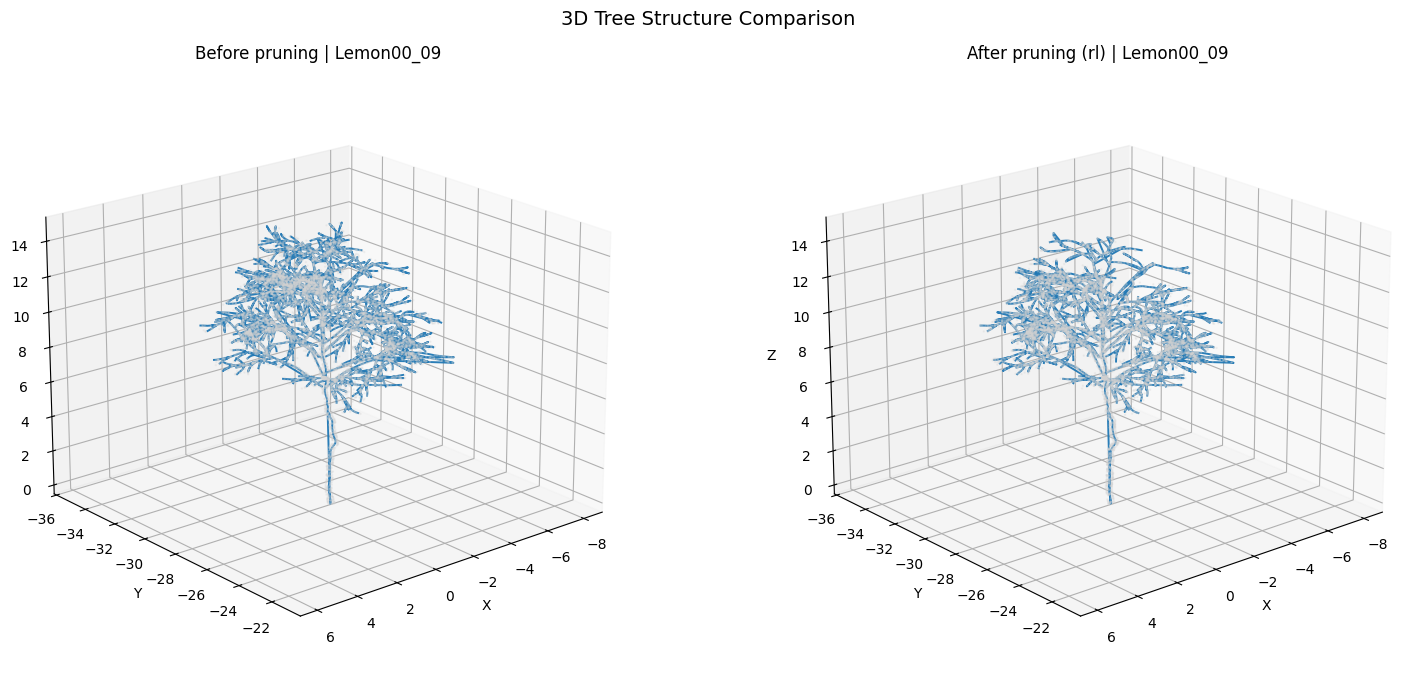
\includegraphics[width=0.78\textwidth]{figures/Tree_structure_comparison.png}
\caption{Global skeleton comparison before and after pruning for sample Lemon00\_09}
\label{fig:tree_3d}
\end{figure}

\begin{figure}[H]
\centering
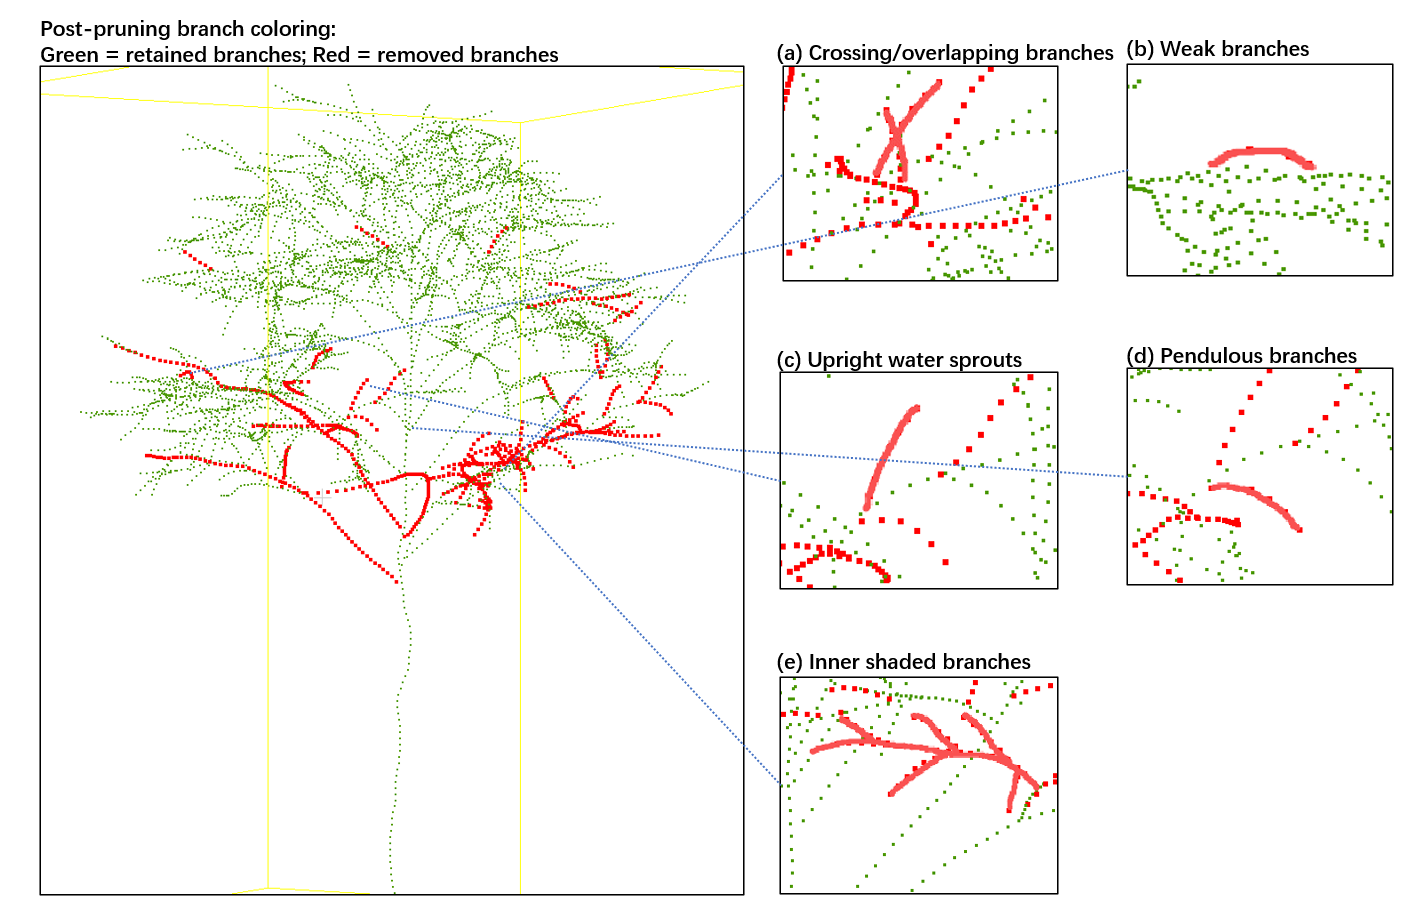
\includegraphics[width=0.98\textwidth]{figures/pruning_categories_eg.png}
\caption{Pruning results for sample Lemon00\_09 and local enlargements of typical removed branch types}
\label{fig:pruning_categories}
\end{figure}



From the whole-tree distribution, removed branches are not spread uniformly across the canopy,
but concentrate where interior overlap, local occlusion, and abnormal branch posture are most pronounced;
the trunk, main scaffold branches, and many peripheral fine branches are retained.
This spatial pattern shows that the learned policy does not aim directly at reducing branch count,
but under root-branch protection, minimum structure constraints, and functional-branch protection,
prioritizes local structural issues that affect interior canopy openness, branch layering, and load-bearing organization.
Improvements in crowding $C$, light accessibility $\mathcal{L}$,
balance $B$, and structural stability $S$ in Table~\ref{tab:single_tree_kpi_change_75}
are not merely the effect of simple thinning,
but rather a composite outcome of screening defective branches by spatial position and structural role.

In Figure~\ref{fig:pruning_categories}(a), red branches are spatially close to  retained neighbors 
and show clear projection overlap, 
corresponding to crossing-branch discrimination logic: 
only non-parent--child pairs exhibiting spatial proximity, directional difference, horizontal projection overlap, and vertical interval overlap 
are treated as structural interference requiring intervention. 
In (e), red branches extend toward the interior, 
a typical inner shaded branch form; 
the issue is not single-branch length per se,
but growth direction bringing occupancy back into the canopy interior, weakening interior illumination.

Another set of examples reflects branch posture and structural quality more strongly.
In (c), removed branches grow nearly vertically upward
with pronounced length, matching upright water sprout criteria;
such branches typically occupy upper space and compete with neighbors for light and nutrients.
In (d), removed branches show clearly pendulous posture,
corresponding to pendulous-branch rules, with low retention value and poor contribution to spatial organization.
In (b), red branches are relatively thin.
Spatially, overall pruning aligns well with the quantitative indicator changes.




% ============================================================
% 第6章 结论
% ============================================================
\section{Conclusion}\label{sec:conclusion}

This paper targets the dormant pruning task of fruit trees and establishes a sequential decision framework that integrates horticultural rules, tree state evaluation, and offline learning. Methodologically, we first formalize defective branches (crossing branches, inner-shaded branches, upright water sprouts, pendulous branches, weak branches) and functional branches (medium-short branches, thick branches) based on 3D skeleton topology and geometric attributes. We then construct a tree evaluation model covering structural hierarchy, crowding, balance, light accessibility, fruit-bearing potential, and structural stability, based on which a composite reward function is designed. Finally, the Decision Transformer is adopted to learn pruning decision policies on offline trajectory data.
Experimental results show that rule-based pruning strategies generally outperform random pruning. Under the same rule conditions, sequential decision-making is more conducive to controlling the loss of fruit-bearing potential caused by excessive pruning compared to batch decision-making. Compared with behavioral cloning and pure rule-based sequential policies, the Decision Transformer demonstrates good comprehensive performance in light improvement, fruit potential control, and termination timing selection.
The work in this paper demonstrates that horticultural experience in fruit tree pruning can be transformed into computable discriminative conditions and state indicators, which can be used to construct decision constraints and evaluation bases required for offline learning. The main contribution of this paper lies in establishing a transformation path from descriptive horticultural knowledge to mathematical decision-making models. For such irreversible, long-cycle agricultural tasks, rule modeling and state evaluation remain important components in decision system design. At the same time, the six indicators adopted in this paper are essentially representative features oriented to the current tree structure, and their correspondence with subsequent measured light, expert ratings, and yield performance remains to be further verified under richer tree species and field observation conditions.


% ============================================================
% 参考文献
% ============================================================
% Appendix
\appendix
\section*{Appendix A. List of Symbols}
\phantomsection
\addcontentsline{toc}{section}{Appendix A. List of Symbols}
\label{app:symbols}

The symbols used in the formulae are summarized in \cref{tab:symbols}.

\footnotesize
\begin{longtable}{>{\raggedright\arraybackslash}p{0.25\textwidth}
                  >{\raggedright\arraybackslash}p{0.67\textwidth}}
\caption{List of symbols used in the formulae}\label{tab:symbols}\\
\toprule
\textbf{Symbol} & \textbf{Meaning} \\
\midrule
\endfirsthead
\toprule
\textbf{Symbol} & \textbf{Meaning} \\
\midrule
\endhead
\bottomrule
\endfoot
$b, b_i, b_j$ & Branch identifiers; $b_0$ denotes the trunk branch. \\
$V, E, G$ & Vertex set, edge set, and branch-level graph of the tree. \\
$\operatorname{parent}(b)$ & Parent branch of branch $b$. \\
$\operatorname{desc}(b)$ & Set of descendant branches of branch $b$. \\
$\mathcal{P}_t$ & Point-cloud representation of the tree at pruning step $t$. \\
$\mathcal{S}_t$ & Skeleton representation of the tree at pruning step $t$. \\
$\mathcal{A}_t$ & Set of prunable candidate actions at step $t$. \\
$a_t$ & Action selected at step $t$; \texttt{STOP} denotes termination. \\
$\mathcal{R}$ & Root-branch set. \\
$\mathcal{B}, \mathcal{B}_t$ & Branch set and legal candidate branch set. \\
$\mathcal{B}_{\mathrm{eff}}$ & Effective branch set after excluding very short branches. \\
$\mathcal{B}_{\mathrm{root}}$ & Branch set used for root-branch protection. \\
$\mathcal{Q}$ & Set of effective non-parent--child branch pairs. \\
$\mathbf{p}_i, r_i$ & Skeleton point and local radius of the $i$th point on a branch. \\
$n_b$ & Number of skeleton points on branch $b$. \\
$L_b$ & Length of branch $b$. \\
$\bar{r}_b$ & Mean radius of branch $b$. \\
$\mathbf{c}_b$ & Spatial centroid of branch $b$. \\
$\mathbf{v}_b$ & Unit growth-direction vector of branch $b$. \\
$V_b$ & Estimated volume of branch $b$. \\
$\varepsilon$ & Small numerical stability constant. \\
$d_{\min}(b_i,b_j)$ & Minimum Euclidean distance between two branch skeletons. \\
$d_{\mathrm{cross}}$ & Proximity threshold for crossing or rubbing branches. \\
$\theta_{ij}$ & Angle between the growth directions of branches $b_i$ and $b_j$. \\
$O_{ij}$ & Horizontal projection-overlap score of branches $b_i$ and $b_j$. \\
$O_{\min}$ & Minimum projection-overlap threshold. \\
$\sigma_{ij}$ & Composite severity score for crossing or overlapping branches. \\
$\sigma_{\min}$ & Minimum severity threshold. \\
$\mathbf{o}$ & Geometric center of the canopy. \\
$\hat{\mathbf{d}}_b$ & Reference direction from the canopy center to branch $b$. \\
$\tau_{\mathrm{in}}, L_{\mathrm{in}}$ & Inward-growth threshold and minimum length for inner-shaded branch discrimination. \\
$\alpha_b$ & Angle between branch direction and the upward vertical direction. \\
$\alpha_{\mathrm{vig}}, \alpha_{\mathrm{drp}}$ & Thresholds for upright water sprout and pendulous branch discrimination. \\
$\bar{L}, \bar{r}$ & Mean branch length and mean branch radius within the effective branch set. \\
$\lambda_{\mathrm{vig}}$ & Length multiplier for upright water sprout discrimination. \\
$L_{\mathrm{wk}}, \kappa_{\mathrm{wk}}$ & Length and radius-ratio thresholds for weak branch discrimination. \\
$\tilde{L}_b^{\mathrm{ms}}$ & Relative length used for medium-short branch protection. \\
$\lambda_{\mathrm{ms,lo}}, \lambda_{\mathrm{ms,hi}}$ & Lower and upper bounds for medium-short branch protection. \\
$\kappa_{\mathrm{st}}$ & Radius-ratio threshold for sturdy branch protection. \\
$H, H_{\mathrm{global}}, H_{\mathrm{main}}$ & Structural hierarchy score and its two components. \\
$H_L, H_R$ & Length-order and radius-order hierarchy scores. \\
$\rho_s$ & Spearman rank correlation coefficient between scaffold height and radius. \\
$M$ & Number of primary scaffold branches. \\
$\mathbf{1}[\cdot]$ & Indicator function. \\
$C$ & Branch crowding score. \\
$B$ & Canopy balance score. \\
$\mathbf{g}_{xy}, \mathbf{t}$ & Horizontal weighted centroid and trunk-base position. \\
$k_B$ & Scale coefficient of the balance score. \\
$\mathcal{L}$ & Light accessibility score. \\
$N_{\mathrm{pen}}, N_{\mathrm{ray}}$ & Number of penetrating rays and total sampled rays. \\
$\theta_b$ & Elevation angle of branch $b$. \\
$\Theta_{\mathrm{fav}}, \Theta_{\mathrm{vig}}, \Theta_{\mathrm{drp}}$ & Elevation-angle intervals for favorable, upright, and pendulous branch postures. \\
$f_\theta, f_L$ & Angle factor and length factor in fruit-bearing potential evaluation. \\
$\delta_{\mathrm{fav}}, \delta_{\mathrm{vig}}, \delta_{\mathrm{drp}}$ & Angle-factor adjustment coefficients. \\
$\tilde{L}_b$ & Relative branch length used in fruit-bearing potential evaluation. \\
$\lambda_1, \lambda_2, \lambda_3$ & Empirical interval parameters for length-factor evaluation. \\
$\delta_{\mathrm{mid}}, \delta_{\mathrm{long}}$ & Length-factor adjustment coefficients. \\
$P_b, P$ & Per-branch and tree-level fruit-bearing potential scores. \\
$S, S_z, S_{xy}$ & Structural stability score and its vertical and horizontal components. \\
$\mathbf{g}, \tilde{z}$ & Three-dimensional weighted centroid and its normalized height. \\
$k_S, w_z, w_{xy}$ & Scale coefficient and fusion weights for structural stability. \\
$R_q, R_i, R_c$ & Branch quality reward, state improvement reward, and constraint penalty. \\
$\omega_{\mathrm{cross}}^{-}, \omega_{\mathrm{cross}}^{+}$ & Reward weights for inferior and non-inferior crossing branches. \\
$\omega_{\mathrm{in}}, \omega_{\mathrm{vig}}, \omega_{\mathrm{drp}}, \omega_{\mathrm{wk}}$ & Reward weights for inner-shaded, upright, pendulous, and weak branches. \\
$\pi_{\mathrm{ms}}, \pi_{\mathrm{st}}, \pi_{\mathrm{main}}$ & Penalties for protected medium-short, sturdy, and main scaffold branches. \\
$\Delta, \Delta_e$ & Indicator change and expected per-step change magnitude. \\
$\mathcal{K}$ & Set of structure- and light-related indicators in the reward function. \\
$I_k, \Delta_k$ & Value and before--after change of the $k$th indicator. \\
$W_k, W_P$ & Weight of the $k$th indicator and fruit-bearing potential loss. \\
$P_{\mathrm{cap}}$ & Per-step cap for fruit-bearing potential loss. \\
$V_{\mathrm{total}}$ & Total branch volume before pruning. \\
$\eta_V, \lambda_V$ & Maximum single-step removed-volume fraction and its penalty coefficient. \\
$R_{\texttt{STOP}}$ & Reward assigned to the termination action. \\
$\eta, N_0, N_f$ & Cumulative pruning fraction, initial branch count, and remaining branch count. \\
$\eta_{\mathrm{lo}}, \eta_{\mathrm{hi}}$ & Ideal lower and upper bounds of pruning fraction. \\
$\eta_{\mathrm{buf,lo}}, \eta_{\mathrm{buf,hi}}$ & Buffer lower and upper bounds of pruning fraction. \\
$\eta_{\mathrm{under}}, \eta_{\mathrm{over}}$ & Under-pruning and over-pruning thresholds. \\
$r_{\mathrm{ideal}}, r_{\mathrm{buf}}, r_{\mathrm{under}}, r_{\mathrm{over}}$ & Termination reward and penalty values. \\
$\phi$ & Dual-path state encoder. \\
$s_t$ & Encoded state vector at step $t$. \\
$\mathcal{D}$ & Offline trajectory dataset. \\
$T$ & Trajectory length. \\
$r_t, \hat{R}_t$ & Immediate reward and return-to-go at step $t$. \\
$f_\theta$ & Parameterized Decision Transformer policy model. \\
$\hat{a}_t$ & Predicted action at step $t$. \\
$\mathcal{J}_{\mathrm{CE}}$ & Cross-entropy training objective. \\
$\mathcal{M}$ & Set of non-padded positions in a training sequence. \\
$\mathbf{z}_t, a_t^*$ & Action logits and ground-truth action at step $t$. \\
$N_a, d_s, d_h$ & Action vocabulary size, state dimension, and hidden dimension. \\
$\rho_b, R_t$ & Horizontal distance from branch centroid to trunk base and tree-scale estimate. \\
$\alpha_0, L^*, \rho^*$ & Greedy-baseline normalization constants. \\
$s_1, s_2, s_3$ & Greedy-baseline geometric sub-scores. \\
$w_1, w_2, w_3$ & Weights of the greedy-baseline sub-scores. \\
$\tau_g, \eta_{\max}$ & Greedy-baseline stopping threshold and maximum pruning fraction. \\
$b_t^{\mathrm{greedy}}$ & Branch selected by the greedy baseline at step $t$. \\
\end{longtable}
\normalsize

% References
\bibliographystyle{elsarticle-harv}
\bibliography{references}

\end{document}
